\documentclass[draft, 10pt]{agujournal2019}
\usepackage{graphicx} % Required for inserting images
\usepackage{url} %this package should fix any errors with URLs in refs.
\usepackage{lineno}
\usepackage{amsmath}
\usepackage{booktabs}
\usepackage{tabularx}

\usepackage{tikz}
\usepackage{graphicx}
\usepackage{lipsum}
\usepackage[inline]{trackchanges} 

%\usepackage{natbib}

\drafttrue
\linenumbers
\usepackage[T1]{fontenc}
\author{Connor Cleary}
\date{January 2024}
\begin{document}
\journalname{Hydrogeology Journal}

% \AddToHook{shipout/background}{
%        \begin{tikzpicture}[overlay, remember picture]
%             \node[rotate=45, scale=20, text=grey!10] at (current page) {\;\;\;\;\;\;\;\;\;\;\;\;\;\; DRAFT};
%         \end{tikzpicture}    
%     }
\justify




 
\title{Exploring the effects of bathymetry and aquitard heterogeneity on submarine groundwater discharge and seawater intrusion at pockmarks} 

\authors{Connor A. Cleary\affil{1,2,3},  Jeremy P. Bennett\affil{4}, David E. Dempsey\affil{1}, Leanne K. Morgan\affil{2}}


\affiliation{1}{Department of Civil and Natural Resources Engineering, University of Canterbury, Christchurch, New Zealand}
\affiliation{2}{Waterways Centre, School 
of Earth and Environment, University 
of Canterbury, Christchurch, New Zealand}
\affiliation{3}{Kōmanawa Solutions Ltd, Christchurch, New Zealand}
\affiliation{4}{INTERA Incorporated}

\noindent \textbf{Keywords:} Numerical modeling, geological uncertainty, offshore fresh groundwater, sea-level rise, Wellington Harbour


\begin{keypoints}
\item Bathymetry causes discharge to concentrate around the edges of wide, shallow pockmarks and at the center of deep, narrow pockmarks
\item Comparing modeled and observed discharges and salinities suggests that the aquitard below the pockmarks is heterogeneous
\item Greatest reduction in discharge under sea-level rise and potential for seawater intrusion expected if preferential pathways are present at the pockmarks
\end{keypoints}


\begin{abstract}
Submarine groundwater discharge at seafloor depressions, known as pockmarks, nourishes coastal ecosystems and can be used to identify offshore fresh groundwater.
However, there are no predictions of how pockmark discharges may be affected by sea-level rise or changing abstraction regimes, and the potential for preferential seawater intrusion through pockmarks is unknown.
We analyzed groundwater flow and transport dynamics using a 3D variable density numerical groundwater model representing the hydrogeological conditions of Wellington Harbour,
New Zealand, including high-resolution bathymetry that allowed for the explicit representation of six pockmarks.
We compared possible pockmark geological structures to understand how they modulate discharge.
For pockmarks that reflect a locally pinched aquitard, localized discharge occurs primarily at the margins of shallow pockmarks and at the center of deeper ones.
In contrast, when pockmarks were modeled using high hydraulic conductivity conduits, the greatest discharge occurred through these conduits.
We compare these findings to salinity and discharge observations from Wellington Harbour and found that a range of geological models were needed to explain all observations,
suggesting a degree of heterogeneity across the pockmarks.
We predicted the response of pockmarks to aquifer depletion and sea-level rise scenarios.
We find that whereas sea-level rise is likely to decrease groundwater discharge, significant aquifer depletion could lead to preferential intrusion through the pockmarks.
The greatest reduction in submarine groundwater discharge and the most considerable seawater intrusion occur through high hydraulic conductivity conduits.
Our results suggest that characterizing pockmarks may be important for the sustainable management of coastal and offshore aquifer systems.
\end{abstract} 

\section{Introduction}

At coastlines worldwide, the seaward slope of terrestrial hydraulic gradients causes fresh groundwater to discharge into the sea \cite{arevalo-martinez_ideas_2023, taniguchi_submarine_2019, moore_effect_2010}.
This flux is important, as it supports coastal ecosystems \cite{burnett_groundwater_2003, moore_effect_2010}.
Submarine groundwater discharge can be diffuse, or focused at submarine springs \cite{taniguchi_submarine_2019},
which occur at a variety of features, including: lava tubes \cite{swarzenski_observations_2017},
fractures \cite{bokuniewicz_direct_2008, taniguchi_temporal_2008}, paleochannels \cite{mulligan_role_2007},
karst cavities \cite{fleury_submarine_2007}, and pockmarks \cite{hoffmann_fresh_2023, schluter_spatial_2004}.
The rate and spatial distribution of submarine groundwater discharge can vary seasonally and through tidal stages
\cite{taniguchi_submarine_2019, lee_submarine_2016, dulai_autonomous_2016}.
If the coastal hydraulic gradient is reversed, the submarine groundwater discharge associated with it would cease,
and subsequent seawater intrusion may lead to salinization of fresh groundwater resources \cite{werner_seawater_2013, taniguchi_submarine_2019}.
Under a reversal of the hydraulic gradient, preferential flow paths previously associated with springs may accelerate the salinization of coastal aquifers \cite{geng_preferential_2020, xu_long_2016, falls_hydrogeology_2005}.

Coastal settlements worldwide anticipate increasing pressure on groundwater resources from abstraction for water supply and industrial purposes, due to population growth and sea-level rise \cite{michael_science_2017, oude_essink_effects_2010}.
This increases the risk of salinization, which is concerning, as coastal aquifers provide fresh water for over one billion people  \cite{ferguson_vulnerability_2012}.
If coastal groundwater levels cannot rise with sea level, the component of fresh submarine groundwater discharge driven by seaward terrestrial hydraulic gradient would decrease \cite{morgan_sea-level_2024}.
This will also decrease the reduction in onshore groundwater head required to reverse flow at submarine springs,
increasing susceptibility to seawater intrusion \cite{werner_classification_2017}.

Pockmarks are depressions on the seafloor formed by the upward flow of gas or groundwater \cite{hovland_significance_2002}.
In the case of groundwater flow, pockmark formation is associated with seafloor sediments being destabilized and kept in suspension by discharge,
which reduces deposition rates and alters the sedimentary structure \cite{micallef_can_2023, zhang_review_2025}.
Pockmarks that are associated with groundwater flow have been identified across the world (Figure \ref{fig:pockmarks_global_map}).
Pockmarks can indicate the presence of offshore fresh groundwater \cite{micallef_offshore_2021, post_offshore_2013, bertoni_seismic_2020, hoffmann_complex_2020}.
Submarine groundwater discharge at pockmarks influences seafloor biogeochemistry and microbial communities \cite{purkamo_impact_2022},
and submarine groundwater springs can also be hotspots for marine biodiversity \cite{burnett_economic_2017, alorda-kleinglass_social_2021}.

Offshore fresh groundwater has been proposed as an alternative water resource; however, seawater intrusion through pockmarks may be a key vulnerability of this resource \cite{bakken_submarine_2012, zamrsky_offshore_2022, gyopari_wellington_2018}.
Likewise, changes in the amount of groundwater discharge at pockmarks due to changes in sea level or terrestrial hydraulic conditions,
or seawater intrusion through pockmarks, may have consequences for surrounding ecosystems \cite{purkamo_impact_2022}.
Despite the potential impact, seawater intrusion through pockmarks and the effect of sea-level rise on discharge at pockmarks has not been previously investigated.
While submarine springs in karstic or volcanic settings may have obvious vents \cite{fleury_submarine_2007, swarzenski_observations_2017},
pockmarks are often found in fine-grained sediments \cite{goff_modern_2019, matciak_pockmarks_2024, hoffmann_complex_2020},
which may make the identification and characterization of any associated preferential flow paths more challenging.

\begin{figure}[h!]
\makebox[\textwidth][c]{\includegraphics[width=1.35\textwidth]{global_map.png}}
\caption{Pockmarks associated with groundwater flow in areas with offshore fresh groundwater or with ecosystems sustained by submarine groundwater discharge. Locations include the Skagerrak \cite{andresen_longevity_2021, hubscher_seismic_2006}, the Baltic Sea \cite{hoffmann_complex_2020, matciak_pockmarks_2024, virtasalo_submarine_2019}, the Corinth Gulf \cite{christodoulou_active_2003}, the Pearl River Delta \cite{sheng_offshore_2023, zhu_types_2021}, the U.S. Atlantic Margin \cite{gustafson_aquifer_2019, goff_modern_2019}, the Canterbury Bight \cite{micallef_3d_2020, micallef_multiple_2022}, and the Wellington Harbour \cite{hoffmann_fresh_2023}. (b) shows the location of observations of low salinity groundwater and pockmarks at Puck Bay, one of two locations in the Baltic Sea. (c) shows the locations of observations of low salinity groundwater and pockmarks at Martha's Vineyard on the U.S. Atlantic Margin. * denotes that the pockmarks are only implicitly related to groundwater flow by their co-occurrence.}
\label{fig:pockmarks_global_map}
\end{figure}

The physical characteristics of pockmarks associated with groundwater flow vary.
They are generally found from within 1 km of the shoreline, e.g. \citeA{virtasalo_submarine_2019}, to more than 100 km offshore at the edge of continental shelves,
e.g. \citeA{goff_modern_2019}. They may be up to 100 m in diameter, and up to 15 m deep \cite{micallef_can_2023}.
Pockmarks may be formed as regular or elongated singular depressions, composite or chained depressions, depressions with a raised eye in their base \cite{hovland_significance_2002},
or contain smaller intra-pockmarks inside of them \cite{hoffmann_complex_2020}.
As well as being sites of submarine groundwater discharge, pockmarks can be associated with submarine landslides and slumps and can indicate fluid overpressure preceding earthquakes \cite{hovland_significance_2002}.

Currently, the only published study modeling groundwater discharge at pockmarks is that of \citeA{kaleris_modelling_2002},
which represented pockmarks by increasing the hydraulic conductivity of the aquitard overlying the coastal aquifer in the vicinity of pockmarks.
They compared the modeled groundwater discharge at two different pockmarks, the impact of including or ignoring variable-density effects,
and sensitivity to the value chosen for the seawater molecular diffusion coefficient.
When density effects were ignored, groundwater was discharged across the entirety of both pockmarks, with more discharge around the edges.
For one of the pockmarks in that study, the focusing of discharge around the edges was much greater, due to differences in the hydraulic conductivity distribution around the pockmarks.
When density effects were modeled, discharge was further displaced to the edges of both pockmarks, and the groundwater flow at the center of the pockmarks depended on the molecular diffusion coefficient, which was used to represent dispersion.
With a low diffusion coefficient, saline groundwater flowed down into the aquifer in the center of the pockmark.
For a high diffusion coefficient, fresh groundwater was discharged across the entire pockmark.
The response of pockmarks to changes in the underlying aquifer conditions, such as the effects of sea-level rise and aquifer depletion, was not considered.

No previous study has represented pockmarks explicitly by including realistic bathymetry and spatially variable aquitard thickness.
We expect that changes in the bathymetry will have a first-order effect on submarine groundwater discharge,
much like the influence of topography on groundwater discharge to surface water bodies, where discharge occurs at changes of slope \cite{winter_relation_1999}.
Modeling of other offshore preferential flow features may provide some indication of the behavior at pockmarks if realistic bathymetry were included.
\citeA{mulligan_role_2007} showed that, for offshore paleochannels, discharge characteristics are controlled by channel geometry and vertical hydraulic conductivity.
In their simulations, channels with wide bases and higher vertical hydraulic conductivity allowed saltwater to descend through the center while freshwater was discharged at the margins.
Conversely, when channel bases were narrower or vertical conductivity was lower, freshwater discharge occurred at the channel center.

In this paper, we model groundwater flow and transport numerically in a cluster of pockmarks in Wellington Harbour, New Zealand.
We consider present-day conditions, sea-level rise, and aquifer depletion scenarios.
We model the pockmarks' geometry and flow dynamics at high fidelity by using high-resolution bathymetry of the harbour,
and compare the effects of different conceptualizations of pockmark geological structure.

Although the model is developed for a specific site, our aim is more general.
This case study aims to act as a well-characterised example to examine how seafloor bathymetry and aquitard heterogeneity together control the location, magnitude, and salinity of submarine groundwater discharge at pockmarks,
and how this discharge responds to sea-level rise and aquifer depletion.
The processes of the study are transferable to the many other settings where pockmarks occur in fine-grained sediments.

While sustained aquifer depletion conditions that would lead to active seawater intrusion are not anticipated in the study location,
they are an imminent concern in many locations around the world \cite{michael_science_2017, ferguson_vulnerability_2012, zamrsky_global_2024}.
Where such conditions coincide with the occurrence of pockmarks} \cite{mendecki_saltwater_2025},
understanding the potential for seawater intrusion through them may be important for aquifer management.

\section{Study area: Te Whanganui a Tara Wellington Harbour}

The Lower Hutt Valley aquifer system is located in the south of the North Island of Aotearoa New Zealand (Figure \ref{fig:pockmarks_wellington_map}).
The aquifer system is an alluvial sedimentary basin that extends 20 km along the Hutt Valley and beneath Wellington Harbour \cite{begg_revised_2023}.
Although the system is relatively small, it is generally representative of coastal unconsolidated groundwater systems,
which make up to 25\% of the global coastline \cite{zamrsky_geological_2020, zamrsky_global_2024}.
The system is recharged by the Hutt River as well as rainfall, and around 15\% of its discharge occurs offshore \cite{bennett_hutt_2024}.
A large proportion of offshore discharge is thought to occur at numerous springs and pockmarks, which are widespread across the harbour \cite{hoffmann_fresh_2023, harding_characteristics_2000}.
The aquifer system supplies on average 40\% of the Wellington metropolitan region's drinking water \cite{begg_revised_2023}.
In the summer, this may be as high as 80\%. A recent offshore exploration project found that offshore fresh groundwater under the harbour was unsuitable as a water source,
due to the risk of seawater intrusion, meaning that protecting the existing onshore groundwater supply is imperative \cite{gyopari_wellington_2018, morgan_likelihood_2022}.

\begin{figure}[h!]
\centering
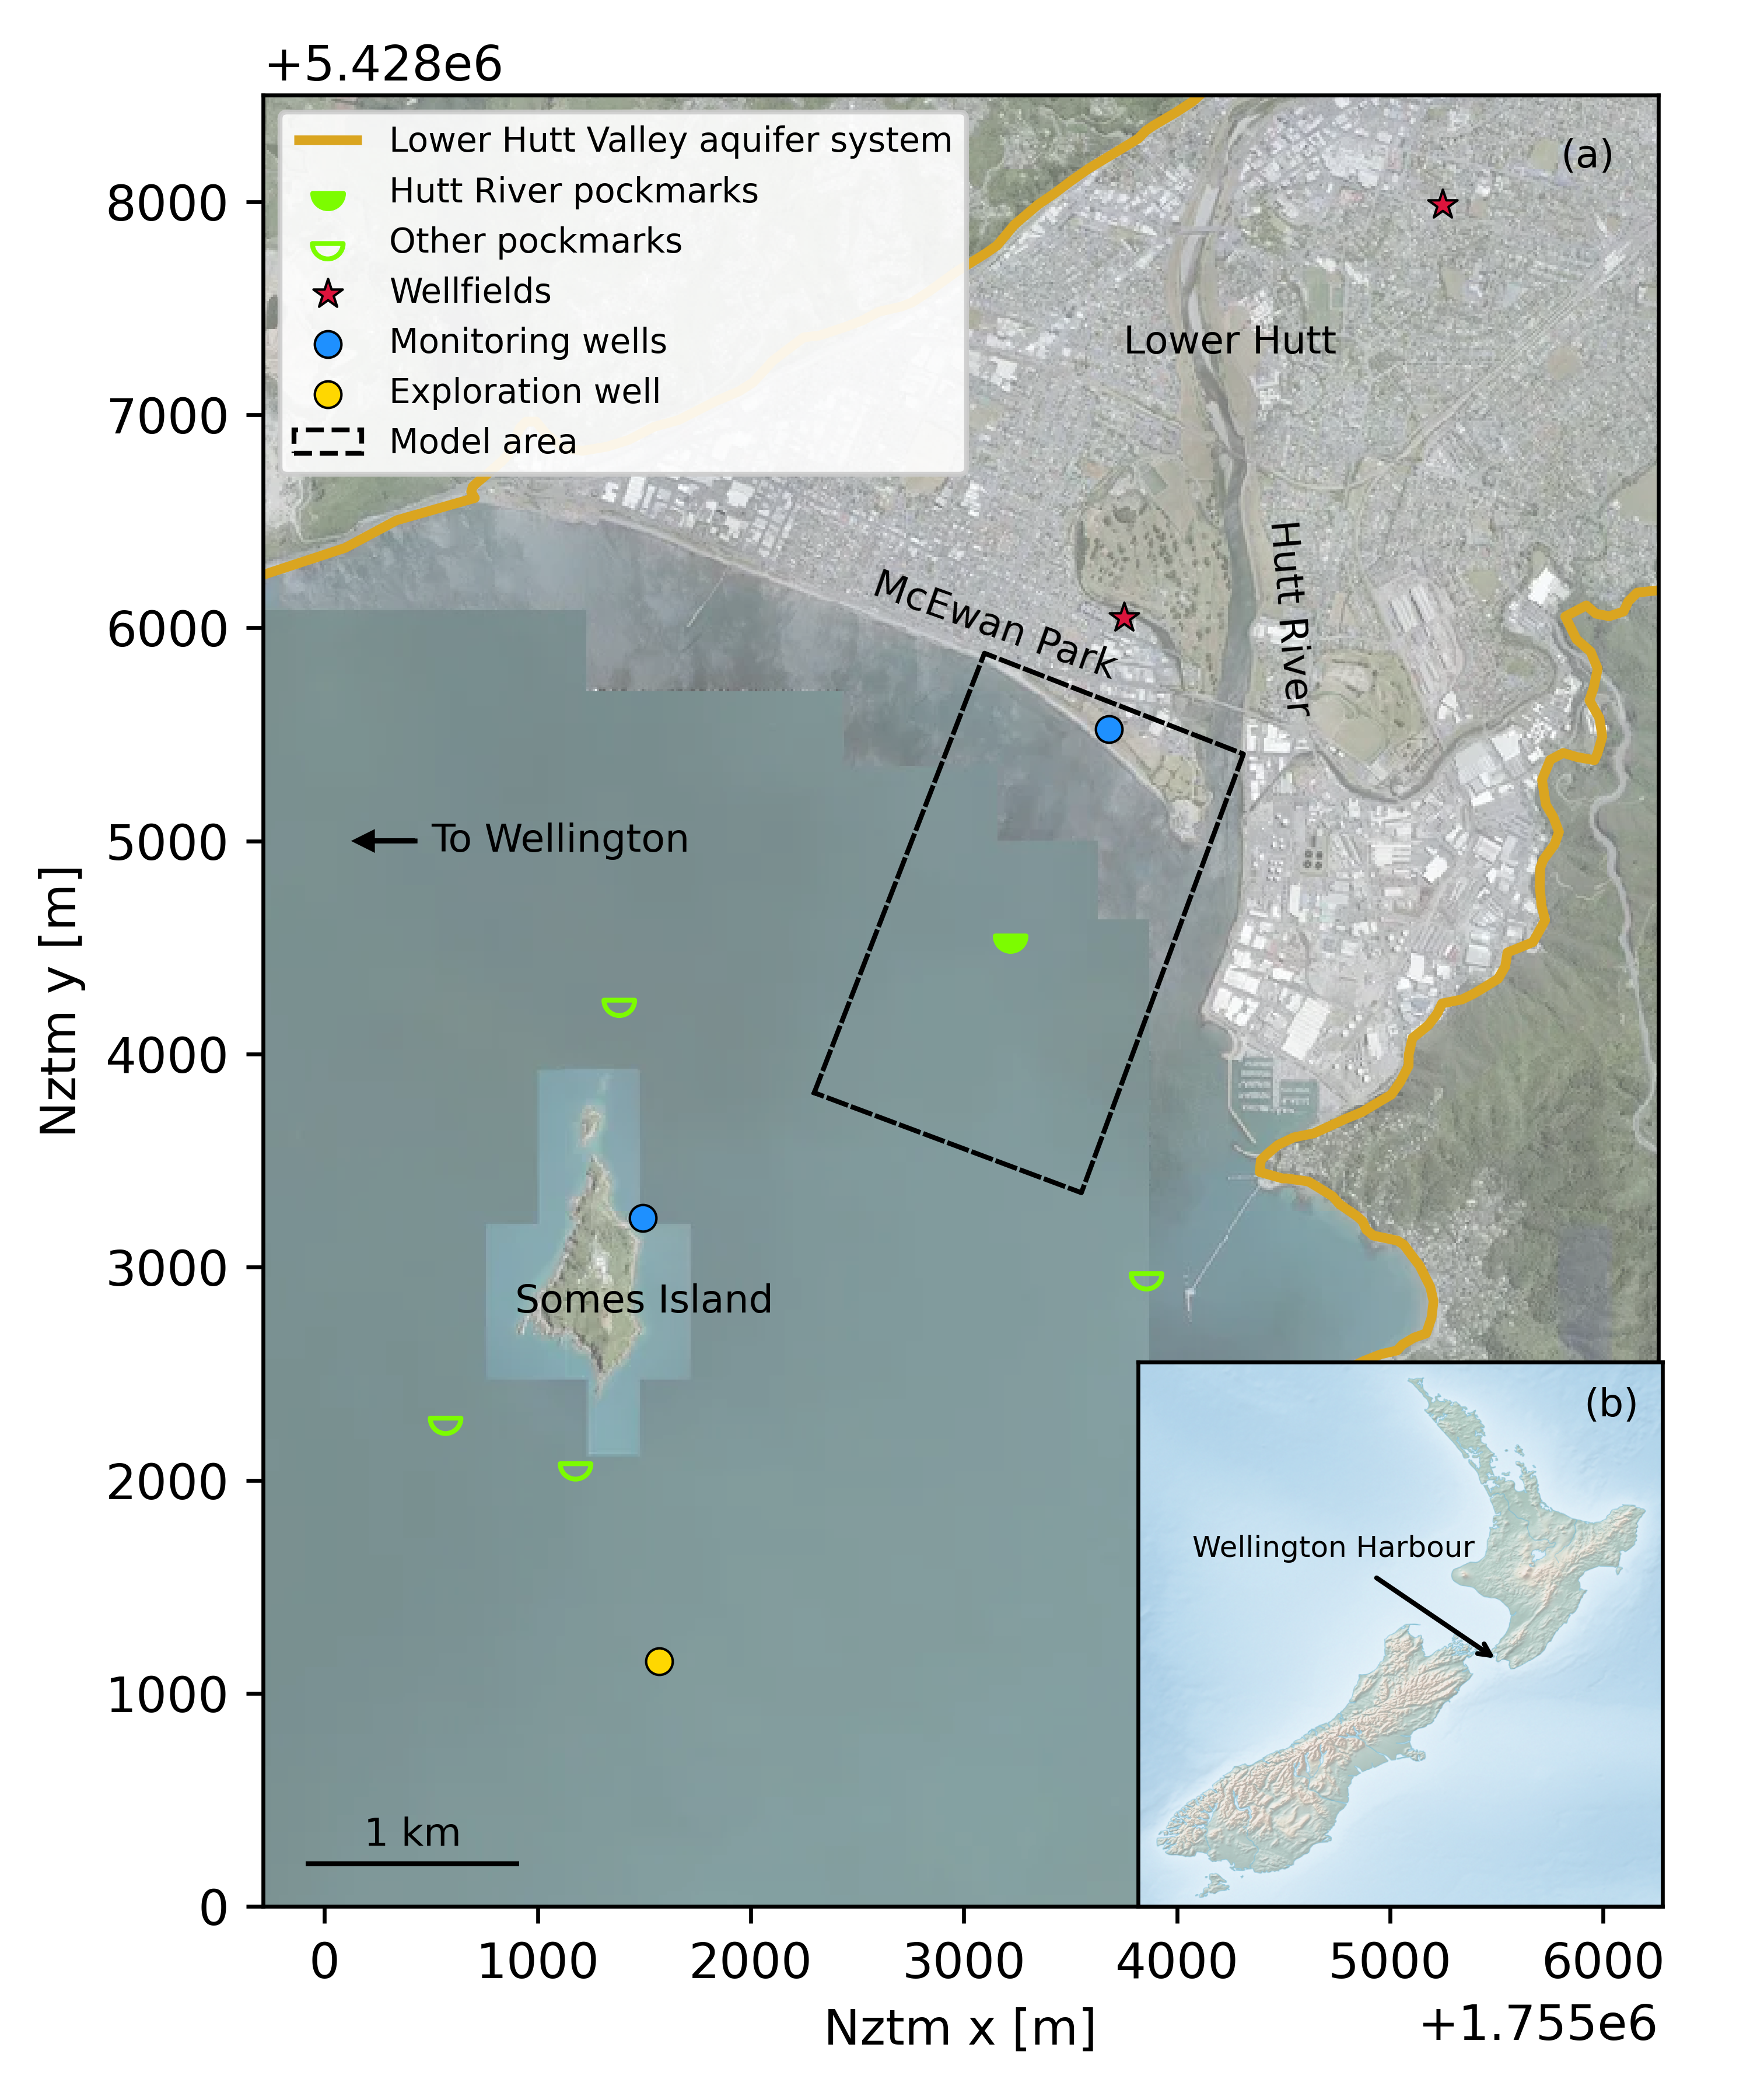
\includegraphics[width=1\textwidth]{map_revision1.png}
\caption{(a) Map of the Wellington Harbour, showing the Lower Hutt Valley aquifer system (outlined in orange). The locations of major pockmarks are shown by green semicircles. The filled green semicircle shows the pockmark cluster studied in this paper. Public supply wellfields are shown with red stars. The two blue circles show two monitoring wells. The black square shows the outline of the study site/model area. (b) Location of the Wellington Harbour in New Zealand.}
\label{fig:pockmarks_wellington_map}
\end{figure}

Because of the proximity of municipal drinking water wellfields to the foreshore, seawater intrusion is a major risk for aquifer management \cite{bennett_hutt_2024}.
To mitigate this risk, monitoring wells along the shoreline are used to ensure the offshore hydraulic gradient is maintained \cite{gyopari_lower_2014}.
Under a reversed hydraulic gradient, it is thought that preferential seawater intrusion could occur through the Hutt River pockmarks,
which are located close to the shoreline (Figure \ref{fig:pockmarks_wellington_map}).
Understanding groundwater flow and salt transport conditions around these pockmarks is crucial to sustainable groundwater management for the Lower Hutt Valley aquifer system,
especially considering the projected sea-level rise and the uncertain future of recharge conditions \cite{michael_science_2017, bennett_hutt_2024}.
Given the importance of this aquifer system, it is an appropriate site to explore the effects of climate change on groundwater discharge at pockmarks and what this means for seawater intrusion vulnerability.

The main aquifer exploited in the Lower Hutt Valley aquifer system is the Upper Waiwhetū aquifer (Figure \ref{fig:pockmarks_info_composite}a). 
The gravel aquifer was deposited during the last glaciation, approximately 30,000 years ago} and is highly transmissive \cite{bennett_hutt_2024, gyopari_lower_2014, shulmeister_timing_2019}.
The aquifer is overlain by the Petone Marine Beds, which consist of three aquitard units, Upper, Distal, and Lower \cite{begg_revised_2023}.
Both the Petone Marine Upper and Petone Marine Lower aquitards comprise gravelly sand, sand, and sandy silt.
The Petone Marine Distal aquitard is significantly less permeable, being composed predominantly of silt and clay.
The marine beds were deposited during the post-glacial Holocene during the last 10,000 year} \cite{gyopari_lower_2014}.

Within the study area, the surface of the Petone Marine Distal aquitard at the seafloor features several pockmarks.
The locations of pockmarks border the offshore extent of the Petone Marine Upper aquitard.
The pockmarks were first observed around 1950, and do not appear to be changing in form over time \cite{harding_characteristics_2000, hoffmann_fresh_2023}.
\citeA{hoffmann_fresh_2023} inferred through their observations that these pockmarks were formed by submarine groundwater discharge, weakening the surface sediments,
which increased erosion by harbour bottom currents. They noted that the Petone Marine Distal aquitard, being close to its onshore extent,
is thinner and likely more heterogeneous at the Hutt River pockmarks, contributing to the localization of groundwater discharge and erosion.
The Hutt River pockmarks are associated with a reduction in the thickness of the Petone Marine Distal aquitard (Figure \ref{fig:pockmarks_info_composite}b).
On average in the study area, the aquitard is estimated to have a thickness of 10 m. At the base of some of the pockmarks, the aquitard may be less than 2 m thick.


\begin{figure}[h!]
\centering
\makebox[\textwidth][c]{\includegraphics[width=1.35\textwidth]{background_composite_revision2.png}}
\caption{(a) Geological model of the study area, containing the hydrostratigraphic units of interest, adapted from \citeA{begg_revised_2023}. Going downward, these are the Petone Marine Upper, Petone Marine Distal, and Petone Marine Lower aquitards, and the Upper Waiwhetū aquifer. On the surface of Petone Marine Distal aquitard, several pockmarks are visible. (b) Interpolated thickness of the Petone Marine Distal aquitard in the study area, based on the pockmark bathymetry and three-dimensional geological model of \citeA{begg_revised_2023}. (c) Proposed geological models of the pockmarks.}
\label{fig:pockmarks_info_composite}
\end{figure}

Two field studies of the Hutt River pockmarks have been undertaken.
\citeA{hoffmann_fresh_2023} took sediment cores from three locations within the study area (Figure \ref{fig:pockmarks_info_composite}b).
Cores MC2-1 and MC2-3, located at the bases of two pockmarks, both had decreasing salinities to a depth of 0.5 m, from 35 PSU to 10 PSU for MC2-1, and from 33 PSU to 17 PSU for MC2-3.
Core MC2-2 was taken at a site between pockmarks, where turbidity and salinity anomalies were detected in the water column.
This core had the lowest salinity, with salinities ranging from 14 PSU to 0.5 PSU over a depth of 0.5 m.

\citeA{harding_characteristics_2000} took measurements of the vertical velocity and salinity of the water column at the base of two of the pockmarks where spring vents were observed,
using a modified instrument for measuring ocean currents (Figure \ref{fig:pockmarks_info_composite}b).
The instrument was fixed inside a cylindrical drum, which was placed on the seafloor, in an effort to isolate the water within from external currents.
At SV1, the velocity was estimated to be 1.4$\times$10$^3$ m/day to 3.6$\times$10$^3$ m/day. Located in a deeper pockmark, the velocity at SV6 was estimated to be 0.6$\times$10$^4$ m/day to 1.2$\times$10$^4$ m/day.
The velocities appeared to be strongly correlated with groundwater levels at the McEwan Park monitoring well.
Water column salinity near the base of pockmarks was between 30 PSU and 33 PSU, with greater salinities being observed at high tide.
This suggests that the pockmark discharge rate is sensitive to the difference in head between aquifer and ocean (which is tidally modulated) and thus potentially vulnerable to aquifer depletion or sea level rise.
It should be noted that the discharge velocity observed at the spring vents exceeds the typical range of values reported in the literature by around one order of magnitude \cite{diego-feliu_combining_2025}.
Hence, observational error should be considered in the interpretation of these measurements, especially given the improvised methodology.

At an exploration borehole further offshore than the study area, the salinity in the Upper Waiwhetū aquifer was observed to be $<$ 2 PSU \cite{gyopari_wellington_2018}.
Regional groundwater modeling indicates that the total pockmark spring discharge across the harbour is around 3000 m$^3$/day \cite{bennett_hutt_2024}.

\section{Methods}\label{methods}

\subsection{Numerical modeling}

Variable-density groundwater flow and salt transport are simulated using the finite-difference numerical solver MODFLOW6 \cite{langevin_documentation_2017},
which solves the conservation of mass (Equation 1), and advection-dispersion (Equation 2) equations in terms of hydraulic head:
\begin{equation} \label{eq:comhead}
-\nabla \cdot \boldsymbol{q}=S_s\frac{\partial h}{\partial t},
\end{equation}
where $S_s$ [1/m] is the specific storage,  and $\boldsymbol{q}$ [m/day] is the Darcy flux, and
\begin{equation} \label{eq:consconc} 
n\frac{\partial C}{\partial t}=\nabla\cdot\left[nD^{\ast}\nabla C\right]-\nabla \cdot \left[\boldsymbol{q} C \right],
\end{equation}
where $n$ [-] is the porosity,   $C$ [kg/m$^3$] is the salt concentration, and $D^*(=8.64\times10^{-5} $) [$\mathrm{m}^2/\mathrm{day}$] is the molecular diffusion coefficient. $\boldsymbol{q}$ is calculated using the variable-density form of Darcy's Law (Equation 3):
\begin{equation}
\boldsymbol{q} = -\boldsymbol{K}\left[ \frac{\rho}{\rho_f}\nabla h +(h-z)\nabla\frac{\rho}{\rho_f}\right],
\end{equation}
where  $\textbf{K}$ [m/day] is the hydraulic conductivity tensor, $z$ [m] is the depth from sea level,  and $\rho$ [kg/m$^3$] is the fluid density.
$\rho$ is a function of the density of freshwater $\rho_f$ [kg/m$^3$] and  $C$: $\rho = \rho_f + 0.7143C$.

 Models are built, run, and post-processed using the Python package FloPy \cite{bakker_scripting_2016}.
An overview of the MODFLOW6 flow and transport solver settings, and time-stepping configuration is given in the Supporting Information Section 1.1.

We have not considered mechanical dispersion, as this is likely to result in unphysical back dispersion,
which would lead to an overestimate of the salt transport rate into the aquitard \cite{smith_mixed_2004, irvine_upstream_2021}.
Consequently, we may underestimate the spreading of saline groundwater that enters the aquifer if the effects of dispersion were to be included.
While some back dispersion may still occur due to numerical error \cite{woods_numerical_2003}, these effects appear to be minimal (Supporting Information Figure 1).

\subsection{Geological model and hydraulic properties}
The MODFLOW6 hydrogeological model used in this study is derived from a geological model of the Hutt Valley and Wellington Harbour \cite{begg_revised_2023}.
This model was built using the Leapfrog geological modeling software \cite{seequent_ltd_leapfrog_2020},
which uses radial basis functions to interpolate inferred contact surfaces between hydrostratigraphic units.
The offshore portion of the model is constrained by offshore and onshore boreholes, including those shown in Figure \ref{fig:pockmarks_wellington_map},
and a series of seismic surveys, which were used to delineate the upper and lower contact surfaces of the Upper Waiwhetū aquifer \cite{stantec_gear_2022, begg_lower_2020}.
However, there is significant uncertainty as to the spatial extent of the modeled hydrostratographic units.
The topography of the geological model (Figure \ref{fig:pockmarks_info_composite}a) was created by merging the nationally available 250 $\times$ 250 m bathymetry \cite{niwa_new_2016} with a 5 $\times$ 5 m multibeam bathymetry survey of the Wellington harbour \cite{hoffmann_fresh_2023}.
Below the Upper Waiwhetū aquifer lies the Mid Waiwhetū Silt and Lower Waiwhetū aquifer units.
The Mid Waiwhetū unit is substantially less permeable than the Upper Waiwhetū aquifer and is expected to isolate the Upper Waiwhetū aquifer from the lower hydrostratigraphic units;
it is therefore an appropriate lower boundary for this modeling study.

The hydraulic properties of the hydrostratigraphic units included in the numerical flow model are taken from a recent update of a longstanding regional groundwater model of the aquifer system,
HAM5 \cite{bennett_hutt_2024}.
Hydraulic properties in the regional groundwater model were calibrated using PEST$\_$HP \cite{doherty_pest_hp_2017}.
The transient groundwater model was calibrated to water levels at 29 wells (including at the offshore monitoring well shown in Figure \ref{fig:pockmarks_wellington_map}),
which included more than 4,000 observations over 25 years.
Given the scale of the HAM5 regional model, with layers ranging from 2 m to 20 m thick, and 200 $\times$ 200 m model grid cells,
areas with pockmarks were represented by increasing the vertical hydraulic conductivity of the Petone Marine Distal aquitard \cite{kaleris_modelling_2002}.
In this study, pockmarks are represented explicitly by including fine-scale bathymetry and model discretization.
The calibrated hydraulic properties from HAM5 for the relevant hydrostratigraphic units in the model area are shown in Table \ref{tab:welly_parameters}.
A constant porosity of 0.35 is assumed.

\begin{table}[h!]
\centering
\caption{Calibrated hydraulic properties \cite{bennett_hutt_2024}}
\begin{tabular}{llll}
\hline
Hydrostratigraphic unit & $K_h$ [m/day] & $K_v$ [m/day] & $S_s$ [1/m]  \\
\hline
Petone Marine Upper aquitard & $0.82$& $0.006$  & $2\times 10^{-5}$ \\
Petone Marine Distal aquitard & $5 \times 10^{-4}$& $1.8 \times 10^{-5}$& $3.1\times 10^{-5}$ \\
Petone Marine Lower aquitard & $1.5$& $0.0094$& $5.5\times 10^{-5}$ \\
Upper Waiwhetū aquifer  & $1000$& $0.1$& $3.1\times 10^{-5}$ \\
\hline
\end{tabular}
\label{tab:welly_parameters}
\end{table}

\subsection{Conceptual geological models of pockmark structure}

The hydraulic properties of the Petone Marine Distal aquitard within the pockmarks are uncertain.
As noted by \citeA{hoffmann_fresh_2023}, the Hutt River pockmarks may be influenced by the heterogeneity of the Petone Marine Distal aquitard in the nearshore area.
This suggests that the Petone Marine Distal aquitard may be more hydraulically conductive in the areas where the pockmarks have formed.
Spring vents have also been noted by both \citeA{harding_characteristics_2000} and \citeA{hoffmann_fresh_2023}.
Spring vents occur in small depressions within the pockmarks.
These depressions are 1 m to 2 m in diameter, are characterized by soft seafloor sediment,
and contain several small discharge sites that are visible as plumes of more turbid water \cite{hoffmann_fresh_2023, harding_characteristics_2000}.

To deal with this uncertainty, in this study, we consider three geological models (Figure \ref{fig:pockmarks_info_composite}c).
These models are conceptual representations of the possible geological heterogeneity and resulting magnitude of preferential groundwater discharge at the pockmarks.
The first is the Thin Aquitard model. In this case, we consider that the hydraulic properties of the Petone Marine Distal aquitard do not change within the pockmarks,
and enhanced discharge arises solely from the thinning of the aquitard.
The other two conceptualizations include a degree of heterogeneity of the aquitard hydraulic conductivity in addition to the Thin Aquitard model.
The second is the Patchy Aquitard model, where the hydraulic conductivity of the Petone Marine Distal aquitard is higher within the area of the pockmarks,
similar to the approach taken by \citeA{kaleris_modelling_2002}.
The final model is the Aquitard Conduits model, where spring vents occur both inside and outside the pockmarks, represented by conduits with very high hydraulic conductivity.

In the Patchy Aquitard model, eight regions of the aquitard are assigned as areas where the vertical hydraulic conductivity of the Petone Distal is increased by a factor of two to $3.6 \times 10^{-5}$ m/day.
This is within the range of expected values for the Petone Distal \cite{bennett_hutt_2024},
and is intended to explore how a small change in hydraulic conductivity can affect submarine groundwater discharge and seawater intrusion.
The eight regions correspond to the six pockmarks identified by \citeA{harding_characteristics_2000}, and the two locations outside of these pockmarks where \citeA{hoffmann_fresh_2023} collected sediment cores.
In the Aquitard Conduits model, six locations are chosen for conduits,
where the horizontal and vertical hydraulic conductivity of the Petone Marine Distal and Lower units is increased to $1$ m/day in one column of model cells.
This hydraulic conductivity value represents the upper end of expected values for high-void ratio silt sediments \cite{zhu_experimental_2021},
which is consistent with the description of the spring vent sites \cite{hoffmann_fresh_2023, harding_characteristics_2000}.
The conduits have a diameter of around 1-2 m \cite{harding_characteristics_2000}.
These correspond to the locations where \citeA{hoffmann_fresh_2023} collected sediment cores,
the three spring vents observed by \citeA{harding_characteristics_2000}.
The locations of patches and conduits are shown in Figure \ref{fig:patches_conduits_locations}.
The hydraulic properties and spatial extent of the patches and conduits are summarised in Table \ref{tab:patches_and_conduits}.

The locations of the patches and conduits are intended to explore whether these features can explain the observations,
and in the case of the spring vents, to represent previously identified features.
Identifying the true distribution of such features is beyond the limits of the available data.
Therefore, the results of the scenarios presented in the study are largely hypothetical and should be used only to identify the general differences between the Aquitard models.

\begin{figure}[h!]
\centering
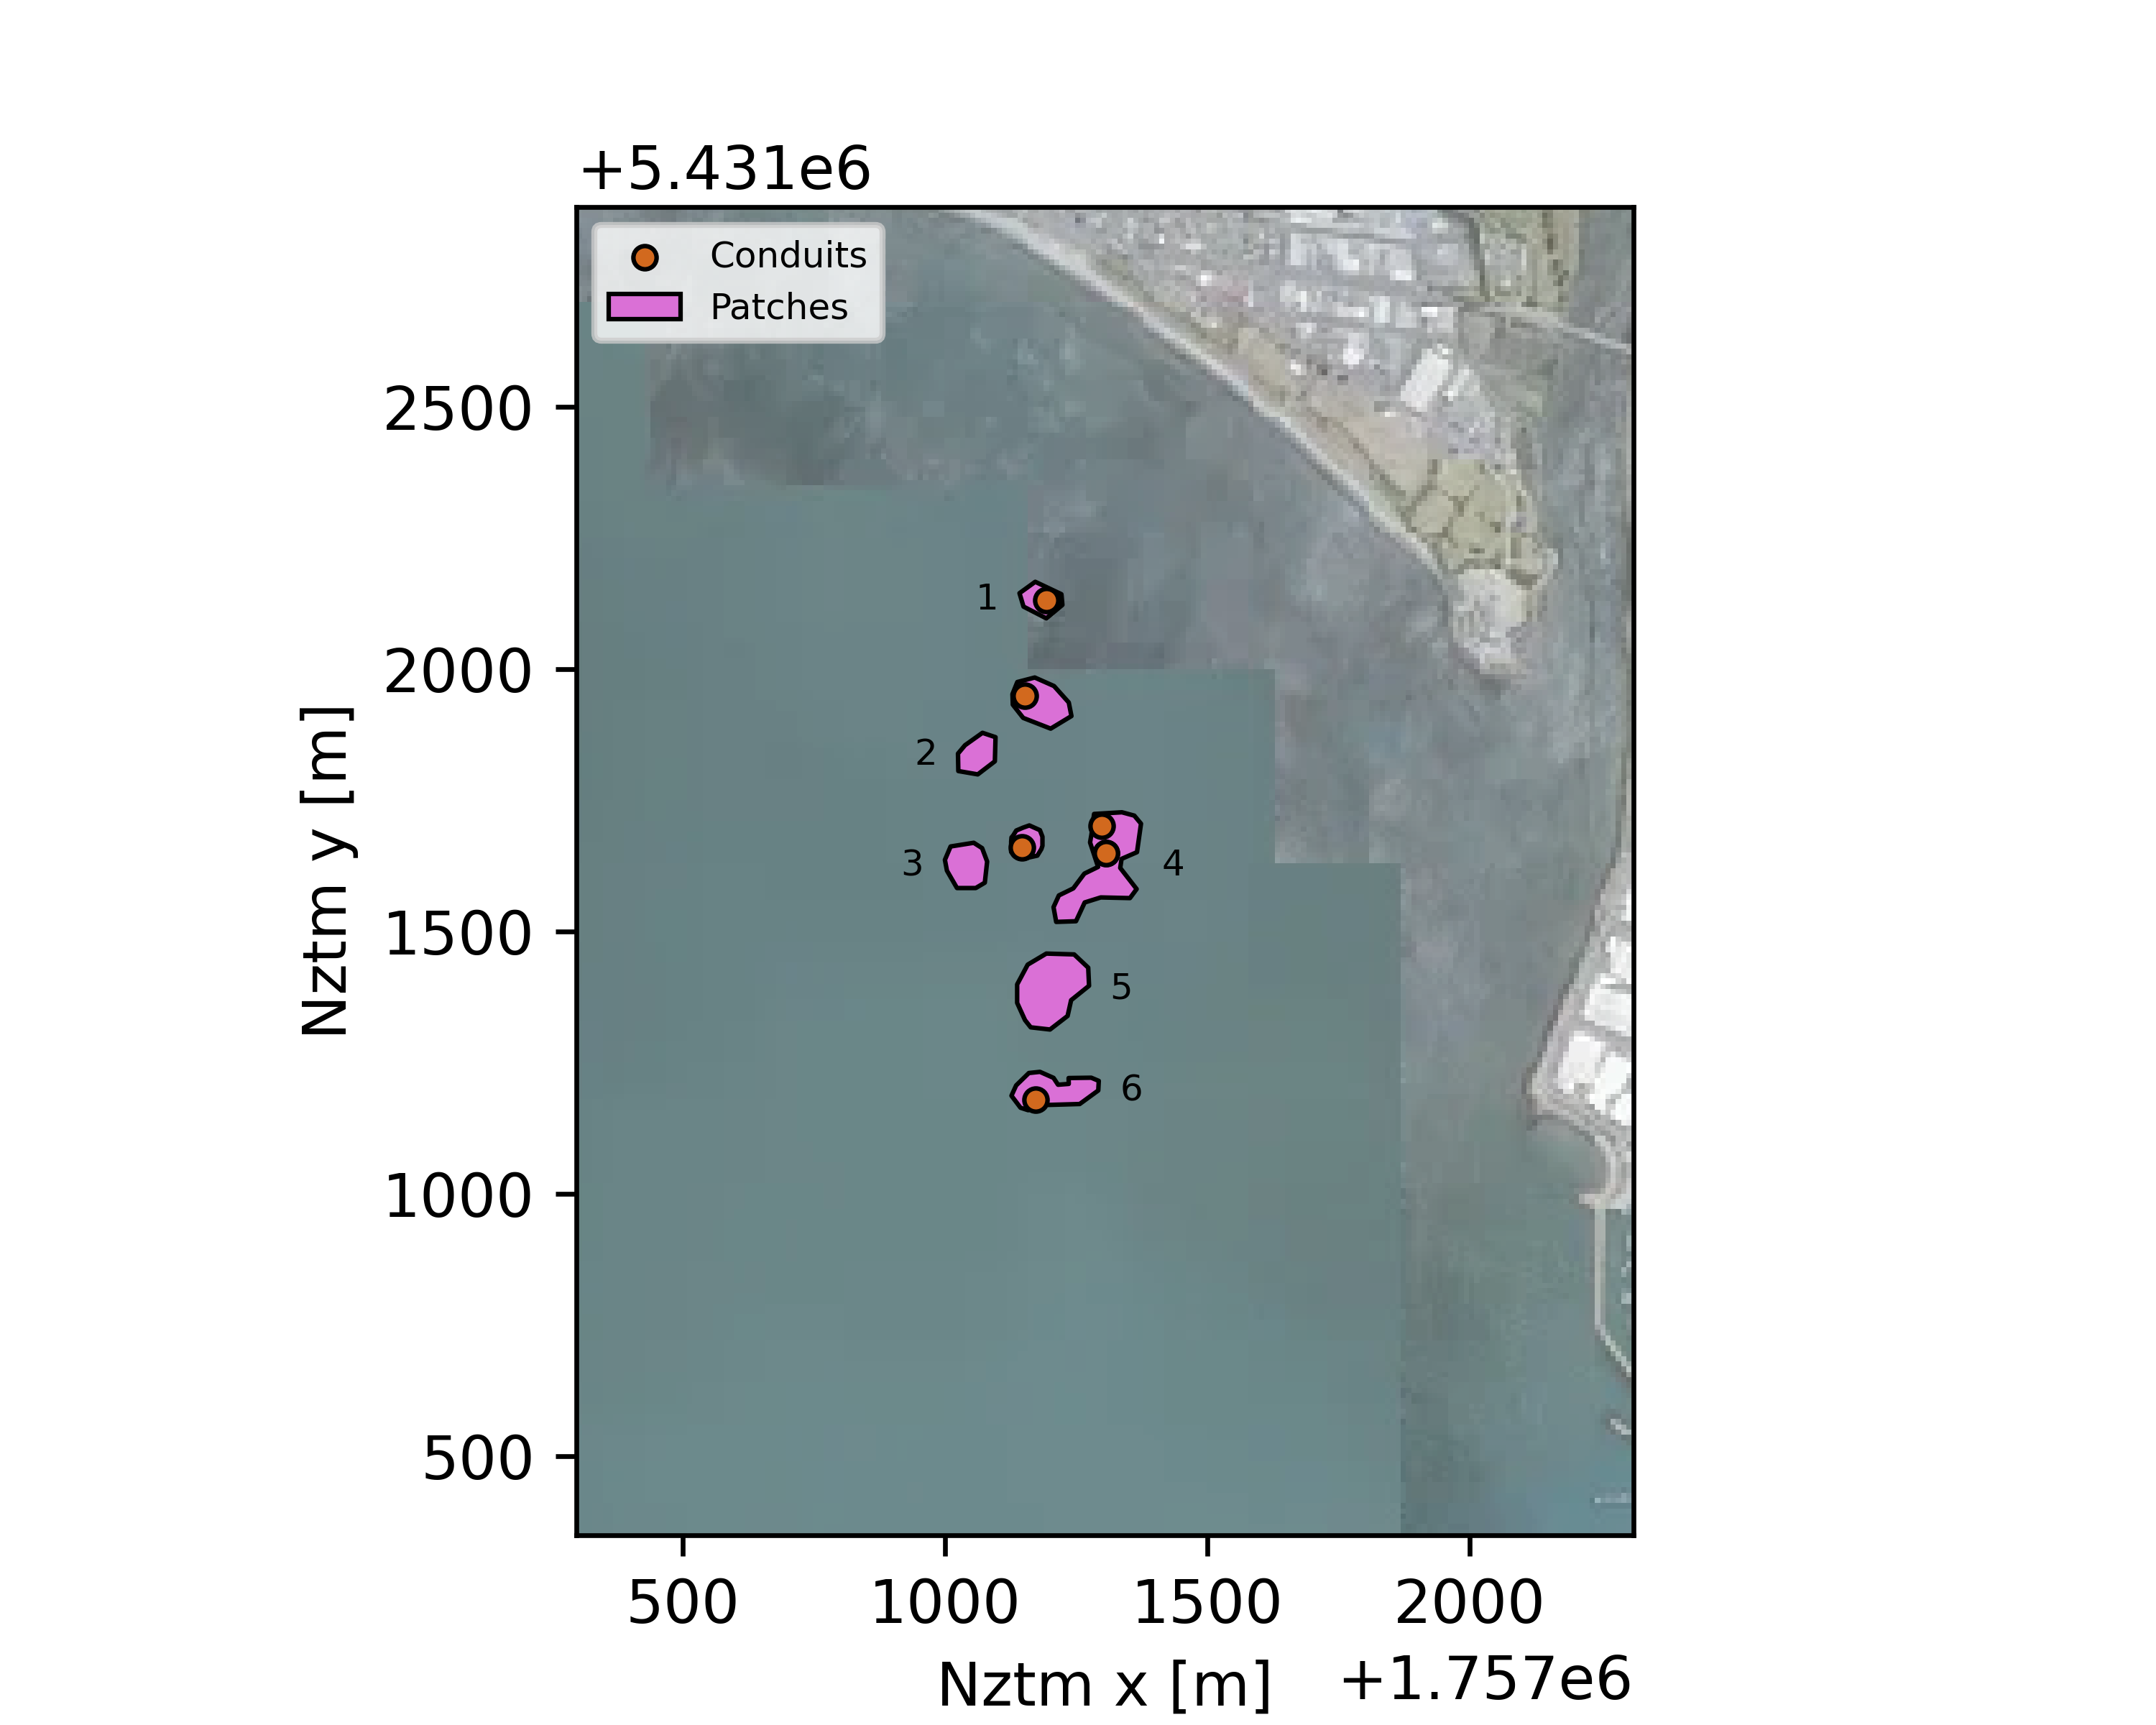
\includegraphics[width=0.5\textwidth]{conduit_and_patches_locations.png}
\caption{Locations of higher hydraulic conductivity patches of the aquitard in the Patchy Aquitard model and conduits in the Aquitard Conduits model. Where these locations correspond to the six pockmarks identified by \citeA{harding_characteristics_2000}, pockmark numbers are shown.}
\label{fig:patches_conduits_locations}
\end{figure}
%%
\begin{table}[h!]
\centering
\caption{Hydraulic properties and placement of the patches and conduits.}
\begin{tabularx}{\textwidth}{l l l l >{\raggedright\arraybackslash}X}
\hline
Feature & $K_v$ [m/day] & Number & Extent & Source \\
\hline
Patch & $3.6 \times 10^{-5}$ & 8 & Pockmark footprint & \citeA{bennett_hutt_2024} \\
Conduits & $1$ & 6 & 1 m to 2 m diameter & \citeA{hoffmann_fresh_2023, harding_characteristics_2000, zhu_experimental_2021} \\
\hline
\end{tabularx}
\label{tab:patches_and_conduits}
\end{table}


These three models are designed as end members rather than as samples from a continuous distribution of aquitard and conduit hydraulic conductivity.
The available data indicate that preferential flow occurs at the pockmarks but do not constrain the volumetric discharge rate.
Additionally, salinity measurements are only available at a two point locations, which are likely to be influenced by fine scale heterogeneity of the aquitard.
A finer sensitivity analysis of patch and conduit conductivity would imply a precision that the observations cannot support, and its results would still depend on the dimensions and internal heterogeneity of the patches and conduits, which are also uncertain.
Were more data to  become available, for example from the geophysical and coring surveys recommended in Section 5.4, a formal sensitivity and uncertainty analysis of these parameters would be warranted.


\subsection{Discretization and boundary conditions}
The discretization of the geological model into a grid for the numerical flow model was carried out in Leapfrog.
The grid is unstructured, and layers follow the hydrostratigraphic structure (Figure \ref{fig:pockmarks_grid}a-b).
Each polygonal element has a diameter of around 10 m, which is reduced to around 1 to 2 m within the pockmarks (Figure \ref{fig:pockmarks_grid}c).
The vertical discretization is dependent on the hydrostratigraphic unit.
The Petone Distal and Upper Waiwhetū aquifer each have 10 layers, and the Petone Upper and Petone Lower each have 5 layers.
Vertical element size ranges between 0.5 m and 2 m. To create a seafloor boundary condition, an extra layer is defined for the seafloor,
which spans the seafloor bathymetry to 2 m above the seafloor.
The thickness of 2 m is to ensure that the grid is continuous across steep areas of the seafloor around pockmarks.
The grid is exported using the Leapfrog Hydrogeology module, then imported into FloPy \cite{hughes_flopy_2024}.
Finally, the thickness of the seafloor layer is reduced to 0.1 m in postprocessing prior to numerical simulation to place the boundary condition as close to the seafloor as possible,
minimizing numerical error. Full grid connectivity is used to improve the accuracy of groundwater flow simulation \cite{provost_accurate_2025}.

\begin{figure}[h!]
\centering
\makebox[\textwidth][c]{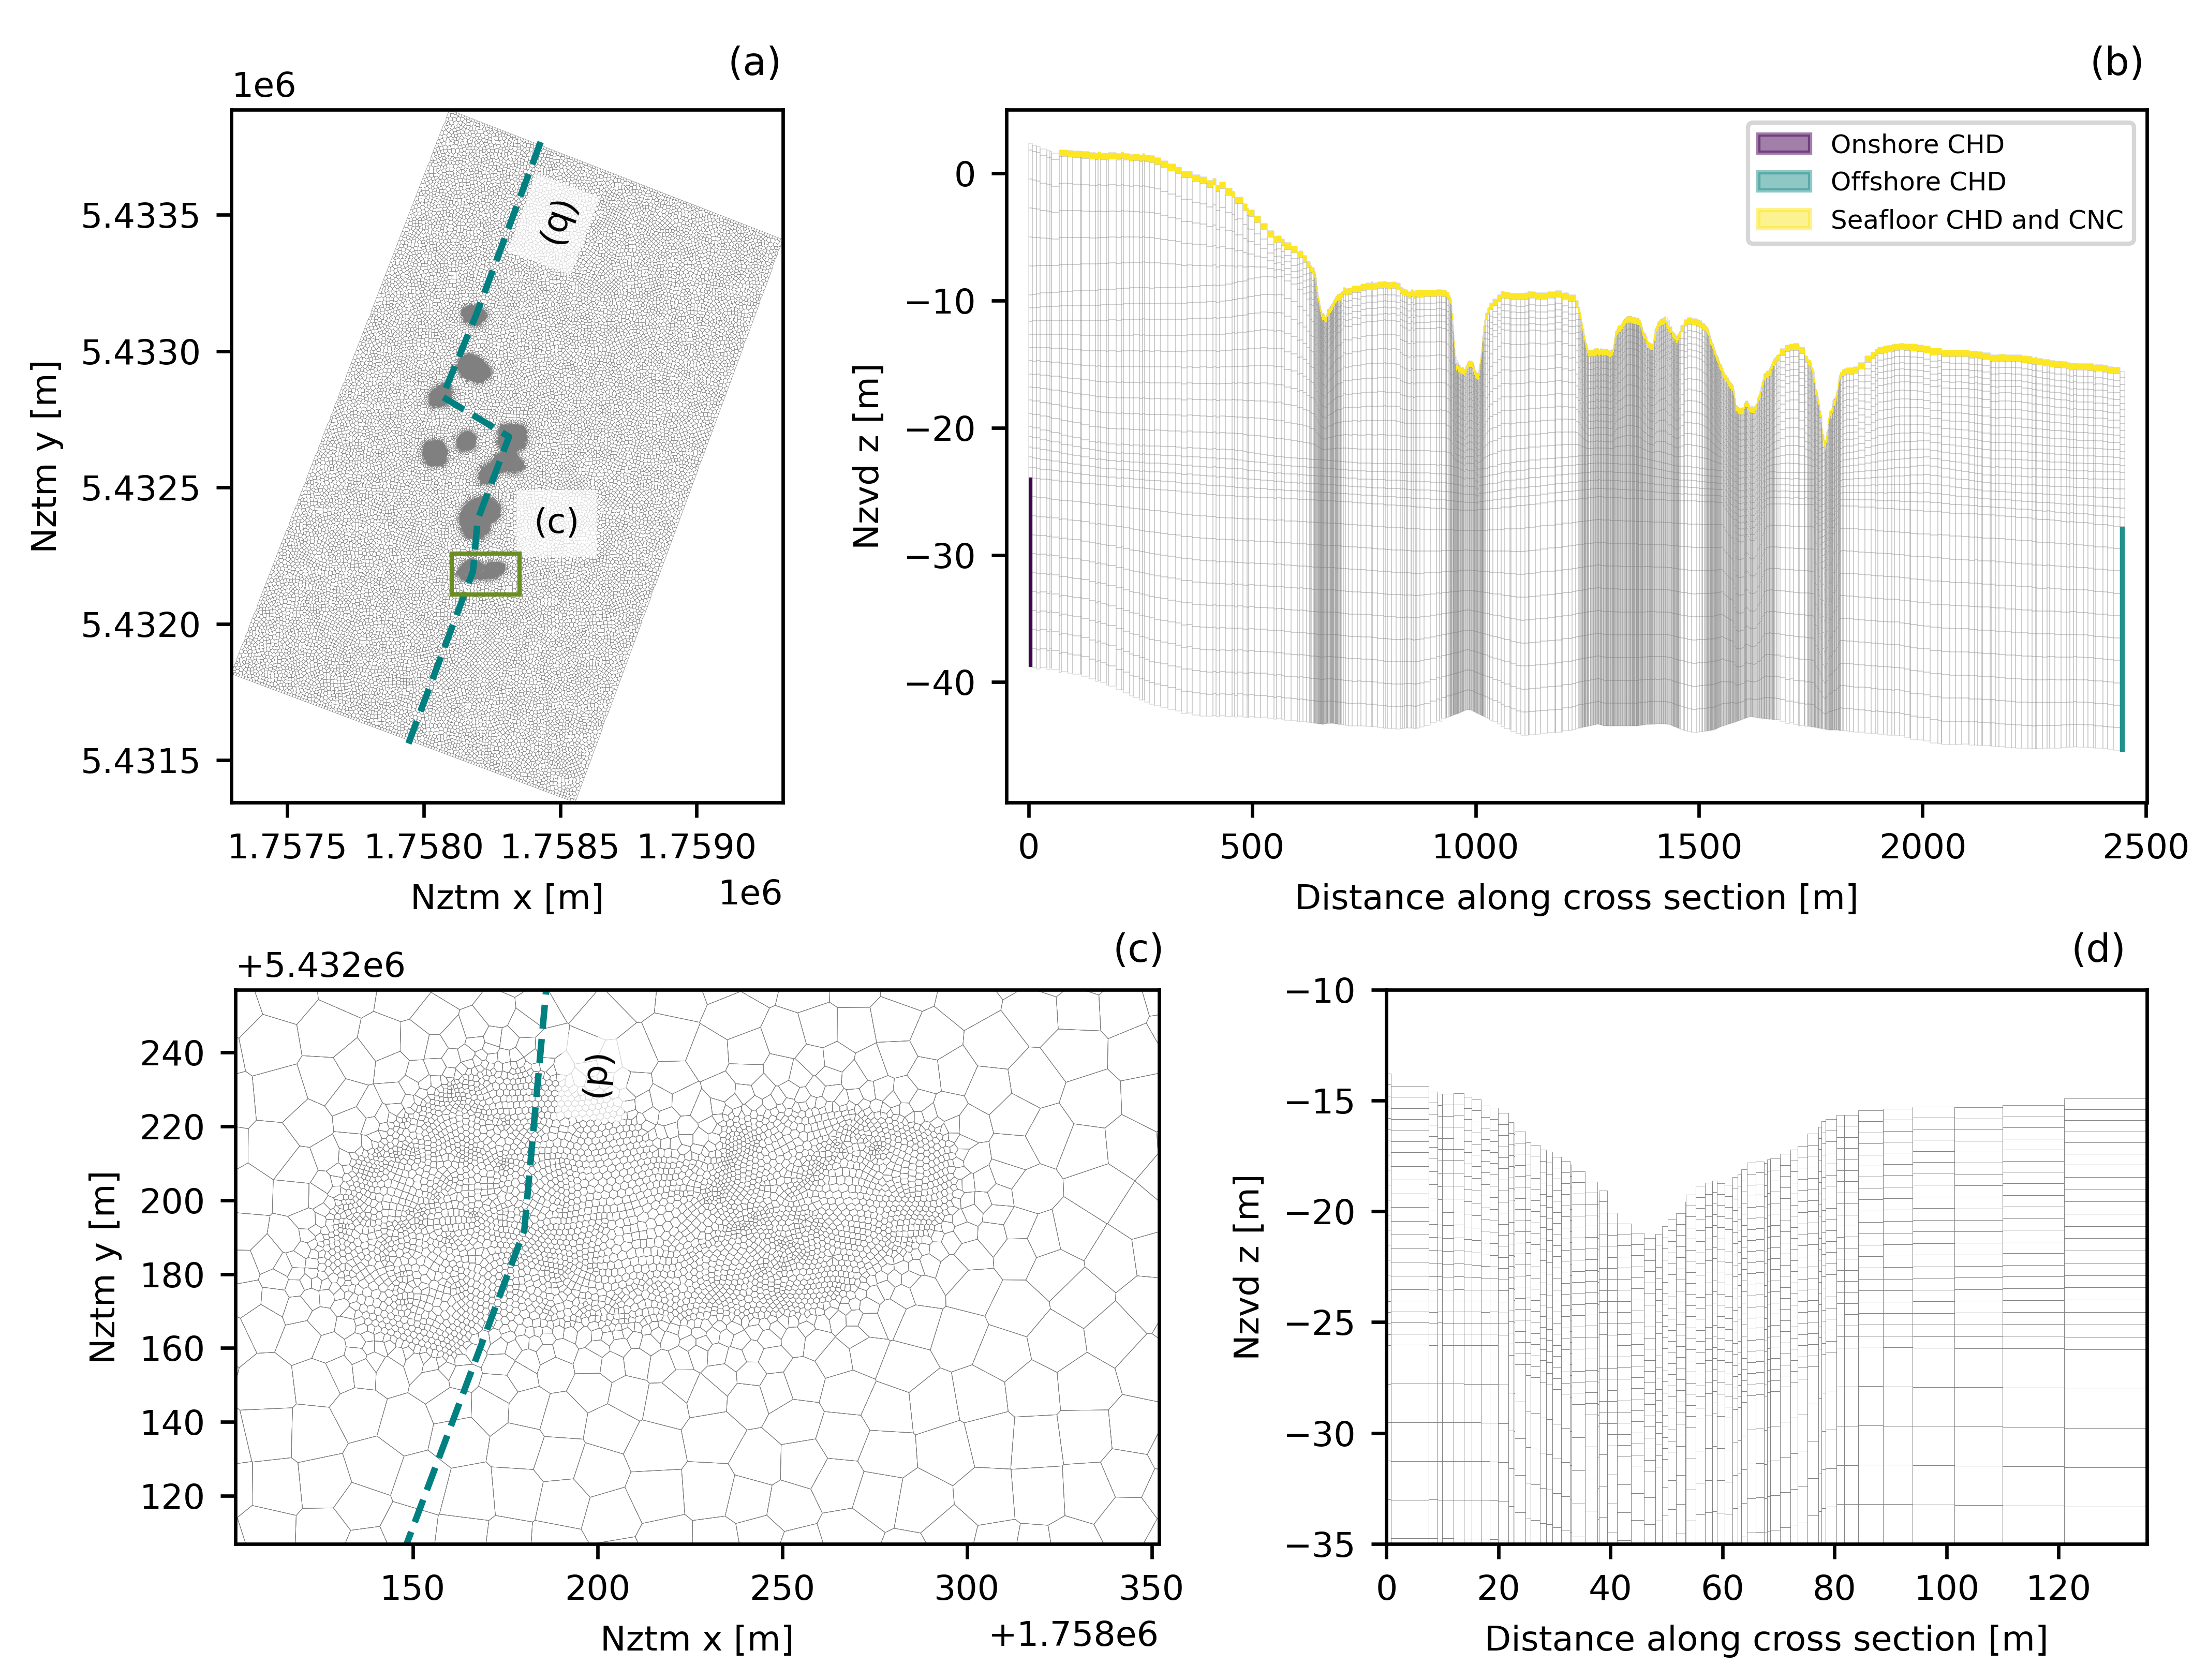
\includegraphics[width=1.35\textwidth]{grid2_boundary_conditions_chd.png}}
\caption{Discretization of model domain and location of boundary cells. (a) Plan view of the entire model grid. (b) cross-section from the shoreline to the offshore extent of the model, which passes through pockmarks. Colored cells show boundary cells. (c) Plan view of a sub-area of the model, showing instructed grid configuration, with local grid refinement in the area of a pockmark. (d) cross-section through the sub-area.}
\label{fig:pockmarks_grid}
\end{figure}

The seafloor boundary is set in all seafloor cells (Figure \ref{fig:pockmarks_grid}b).
The boundary conditions used are a constant head boundary condition (CHD), and a constant concentration boundary condition (CNC).
The ascribed hydraulic head at the seafloor ($h_{\mathrm{sea}}$) depends on the sea-level scenario (Section 3.5), and the constant concentration is 35 PSU, that of seawater.
There are also boundaries at the onshore and offshore extents of the Upper Waiwhetū aquifer, which are used to create the hydraulic gradient through the aquifer.
These two boundaries also use a CHD boundary condition, with a time-invariant constant head (no tidal effects).
The concentration of any water that enters the model at these boundaries is 0 PSU, that of freshwater.
This has been chosen because the Upper Waiwhetū aquifer is known to be fresh further offshore than the model domain,
as shown in Figure 2.1 and Table 5.7 of \citeA{gyopari_wellington_2018}.
This means that salt can only enter the aquifer through the seafloor boundary, which is the focus of this study.
The head value at the onshore CHD boundary ($h_{\mathrm{on}}$) represents the onshore groundwater level, which varies between scenarios.
The head value at the offshore CHD boundary ($h_{\mathrm{off}}$) is prescribed from known predetermined hydraulic gradients,
which are described in Section \ref{scenarios}, given $h_{\mathrm{on}}$.

\subsection{Scenarios}\label{scenarios}
The rates of submarine groundwater discharge at the pockmarks and the salinity of the groundwater below the pockmarks are analyzed for three scenarios of the numerical model (Table \ref{tab:table_stages}).
The first scenario is the present-day average summer groundwater conditions, the second scenario is the estimated groundwater conditions in 2130,
and the third scenario simulates aquifer depletion.

The present-day scenario corresponds to when \citeA{hoffmann_fresh_2023} took observations of porewater salinity in sediment cores and water column salinity.
The future scenario reflects the predicted average summer groundwater conditions in 2130 from the HAM5 regional model.
The HAM5 regional model simulated groundwater heads in the aquifer system in 2130 under a relative rise in sea-level that includes the effects of vertical land movement,
based on the Shared Socioeconomic Pathways scenario SSP5-8.5 \cite{bennett_hutt_2024}.
Also included in HAM5 are the expected changes to the Hutt River and its connection to the groundwater system due to a planned river engineering project.
The outputs of HAM5 used to inform the model presented here are the heads at the two monitoring wells shown in Figure \ref{fig:pockmarks_wellington_map},
which are located in the Waiwhetū aquifer.

The aquifer depletion scenario simulates an extreme case of onshore head reduction.
The onshore head in this scenario is around 2.75 m below the current head limit for aquifer management and protection, and is unlikely to occur in reality.
This is because extraction volumes from this aquifer are actively management with groundwater trigger levels.
However, in this numerical study, it allows for the simulation of hypothetical seawater intrusion into the aquifer.


\begin{table}[h!]
\centering
\caption{Lengths and boundary conditions values of the three scenarios. All heads are given with reference to the New Zealand Vertical Datum. IC refers to the initial salinity conditions in the model. Where the initial conditions are taken from a previous scenario, the scenario number is shown.}
\begin{tabular}{lllllll}
\hline
\# & Scenario & IC &Length [days] & $h_{\mathrm{sea}}$ [m] & $h_{\mathrm{on}}$ [m] & $h_{\mathrm{off}}$ [m] \\
\hline
1 & Present-day & Fresh & $1\times 10^{6}$& $-0.14$  & $2.76$ & $2.64$\\
2 & Sea-level Rise (2130) & 1 & $3.8\times 10^{4}$ & $1.45$  & $2.95$ & $2.88$\\ 
3 & Aquifer Depletion & 1 & $365$& $-0.14$  & $-1$ & $-0.96$\\
\hline
\end{tabular}
\label{tab:table_stages}
\end{table}

The length of the Present-day scenario, 1$\times10^6$ days, was chosen to allow the model to converge on steady-state conditions.
This was found by running the model until no changes in head or salinity were detected.
The value for $h_{\mathrm{sea}}$ reflects the elevation of present-day sea level in the New Zealand Vertical Datum (NZVD).
The value for $h_{\mathrm{on}}$ is based on the modeled average summer groundwater level at the McEwan Park monitoring well from HAM5, which is located at the onshore boundary (Figure 2).
The value for $h_{\mathrm{off}}$ is based on the modeled hydraulic gradient between the McEwan Park and Somes Island monitoring wells in HAM5.
The initial salinity for the Present-day scenario is that of fresh water (0 PSU).

The length of the Sea-level Rise (2130) scenario represents a 105-year period.
The initial conditions for this scenario are taken from the steady-state conditions at the end of the Present-day scenario.
At the end of these 105 years, the model may not have reached a new steady-state, and head and salinity distributions may still be equilibrating with the updated forcing conditions \cite{lu_timescales_2013}.
The value for $h_{\mathrm{sea}}$ reflects the predicted sea level elevation in NZVD, based on the Shared Socioeconomic Pathways scenario SSP5-8.5 \cite{nzsearise_takiwa_2023}.
The value for $h_{\mathrm{on}}$ is based on the modeled average summer groundwater level at McEwan Park under this sea-level rise scenario from HAM5 \cite{bennett_hutt_2024}.
The value for $h_{\mathrm{off}}$ is based on the modeled hydraulic gradient between the McEwan Park and Somes Island monitoring wells, again based on this sea-level rise scenario.

The length of the Aquifer Depletion scenario reflects a possible situation where low aquifer heads are maintained for an extended period of one-year \cite{gyopari_lower_2014}.
Again, the initial conditions for this scenario are taken from the Present-day scenario.
The value for $h_{\mathrm{on}}$ was chosen to force seawater intrusion to occur.
The value for $h_{\mathrm{off}}$ is based on the modeled hydraulic gradient between the McEwan Park and Somes Island monitoring wells, based on the modeled response of the aquifer to depletion \cite{gyopari_lower_2014}.
Note that in this scenario, groundwater flows landward, rather than seaward, like in the previous scenarios.

This scenario is intended as a bounding case that forces flow reversal at the pockmarks, rather than as a forecast of expected conditions.
A head reduction of this magnitude is larger than that permitted under current aquifer management, which maintains a seaward gradient at the shoreline monitoring wells \cite{gyopari_lower_2014},
and would require abstraction well beyond present rates.
We chose a deliberately severe reduction so that the potential for preferential intrusion through the pockmarks could be examined under the conditions where it is most likely to occur.
A shorter or milder depletion would produce correspondingly less intrusion.
A longer period of reversed gradient would allow saline groundwater to penetrate further, as explored for a sustained reversal in the Supporting Information in order to provide insight for other locations where long-term aquifer drawdown is more likely.

\subsection{Comparison of modeled flux and salinity to observations}
The simulated groundwater flux and salinity from each of the models are compared to the two flux observations \cite{harding_characteristics_2000},
and three salinity observations \cite{hoffmann_fresh_2023}. The following assumptions have been made in the comparison between the numerical model and the observations.

The flux observations were recorded as the vertical velocity of the water column,
which was taken in a cylindrical drum placed over the discharge sites \cite{harding_characteristics_2000}.
We assume that at the time of measurement, this cylinder contained solely discharged groundwater which flowed uniformly upwards.
This ignores any interaction between the overlying seawater and less dense plumes of discharged groundwater.
This also ignores the velocity variation caused by many small plumes of discharged groundwater, which have been observed \cite{harding_characteristics_2000}.
Hence, we treat the observed flux as being equivalent to the vertical groundwater flux in the uppermost layer of the Petone Marine Distal aquitard in our model.

The salinity observations are profiles of salinity over 0.5 m deep sediment cores \cite{hoffmann_fresh_2023}.
We assume that the salinity in these profiles is driven only by uniform vertical groundwater flow.
This ignores the effects of horizontal groundwater flow and pore-scale groundwater dynamics, such as preferential flow paths, and porewater exchange \cite{taniguchi_submarine_2019}.
Hence, we consider the average salinity in each 0.5 m deep profile to be equivalent to the salinity in the uppermost layer of the Petone Marine Distal aquitard in our model,
which is also 0.5 m deep. We chose not to compare the full salinity profiles of \citeA{hoffmann_fresh_2023}, which included points at around 10 depths that were unevenly spaced at increments of around 0.05 m,
as this would have required much finer vertical discretization, further increasing the computational burden.
Additionally, making comparisons between measurements at the centimetre-scale in a groundwater model at the metre to kilometre scale is not expected to provide a meaningful insight,
especially given the inherent uncertainty in bathymetry and the assumption of lithographically uniform hydraulic properties beneath the measurement points.

Comparing the salinity in the upper cell of the model to observations may be misleading if the model results contain numerical diffusion error arising from the coarseness of the grid.
However, a comparison of concentration profiles in simplified models with 0.5 m and highly resolved 0.01 m vertical discretization, across a range of fluxes, aquitard thicknesses, and hydraulic conductivities,
suggests that numerical diffusion error is minimal in the models used in this study (Supporting Information Figure 1).

To reduce the impacts of error in the location data for the observations, and of any numerical error caused by the discretization scheme,
we measure the flux and salinity in cells located within a 10 m radius of the observation, for the Thin and Patchy Aquitard models.
For the Aquitard Conduits model, we only consider the cells where the observations are located, as this is where the conduits have been placed.


\section{Results}

\subsection{Effect of bathymetry on submarine groundwater discharge}

To understand the potential influence of bathymetry and the associated thinning of the Petone Marine Distal aquitard at the pockmarks,
the submarine groundwater discharge conditions for the Present-day scenario with the Thin Aquitard model are assessed.
The results from the Thin Aquitard model were chosen to isolate the influence of bathymetry from that of the heterogeneity of aquitard hydraulic conductivity.
These effects are explored using the Patchy Aquitard and Aquitard Conduits models in Section 4.2,
and distributions of groundwater salinity and discharge are shown for the Patchy and Conduit models for all six pockmarks in Supporting Information Figures 2 and 3.

Across the offshore area of the model, groundwater discharges through the Petone Marine aquitards into the Wellington Harbour (Figure \ref{fig_pockmarks_present_day}).
Because the upward flux is small, salt diffuses downwards into the aquitards \cite{jiao_reconstructed_2015}.
As a result, the groundwater, which is of terrestrial origin, reaches the seafloor with a salinity between freshwater and seawater.
The distributed discharge rate across the seafloor (not including the pockmarks) is 13 m$^3$/day, which occurs over an area of around $29 \times10^{5}$ m$^2$,
and has an average salinity of 29.1 PSU.
The discharge rate from the six pockmarks is 0.59 m$^3$/day, occurring over an area of around $0.6\times10^{5}$ m$^2$,
with an average salinity of 25.8 PSU.
This submarine groundwater discharge represents around 1\% of the total amount of groundwater that discharges from the model at the 1.3 km long offshore boundary.

\begin{figure}[h!]
\centering
\makebox[\textwidth][c]{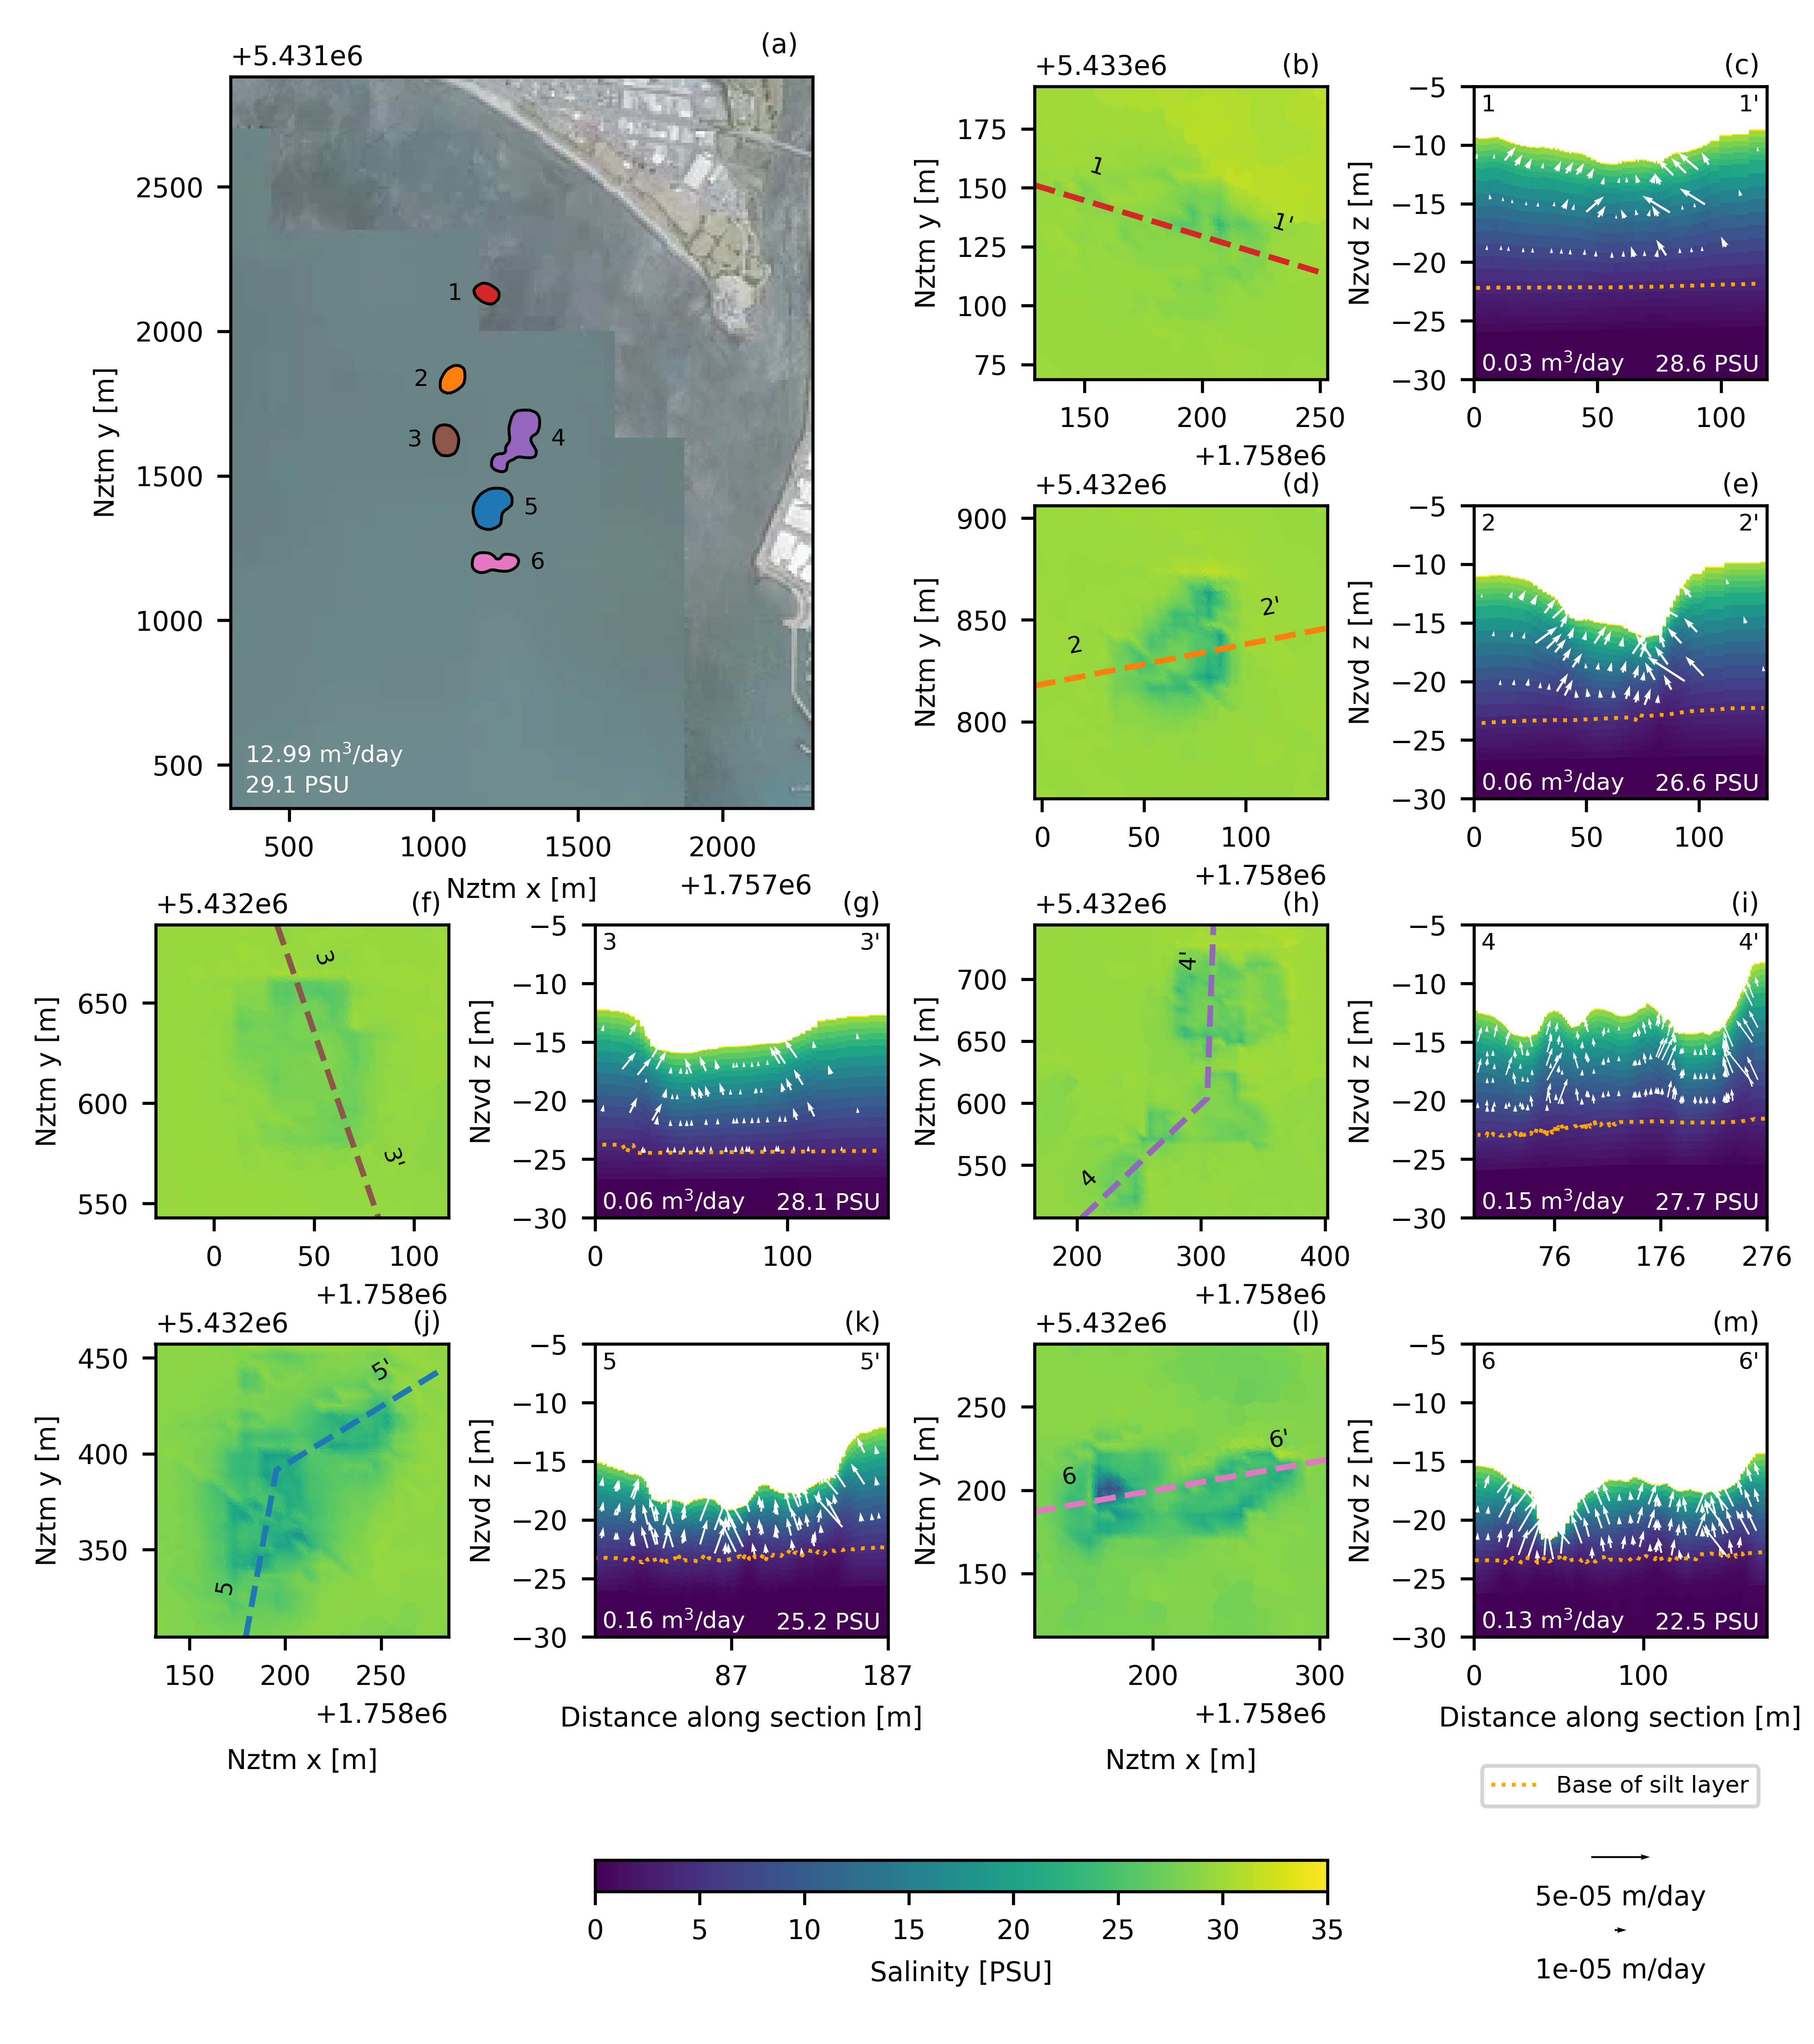
\includegraphics[width=1.1\textwidth]{1average_pockmark_salinity_revision1.png}}
\caption{Modeled salinity distributions and discharge at six pockmarks for the present-day using the Thin Aquitard model. (a) the location of the pockmarks, with white text denoting the rate and salinity of discharge outside of the pockmarks. (b, d, f, h, j, l) the salinity in the uppermost layer of the aquitard, directly below the seafloor. (c, e, g, i, k, m) the salinity and discharge vectors in cross-section for each pockmarks. Vector arrows are shown in the Petone Distal cells. White text denotes the rate and salinity of discharge within each pockmark.}
\label{fig_pockmarks_present_day}
\end{figure}

Compared with the submarine discharge in a 50 m buffer outside of each pockmark, specific discharge was 1.6 (at Pockmark 3) to 2.5 (at Pockmark 6) times greater within pockmarks (Supporting Information Table 1).
Similarly, the salinity of groundwater discharge at the pockmarks was between 3 \% (at Pockmark 1) and 25 \% lower (at Pockmark 6) when compared to the seafloor around them.

This 50 m buffer was chosen based on visual inspection of the typical distance between pockmarks, to avoid overlap with neighbouring pockmarks.
A different buffer distance would likely change the magnitude of the difference in specific discharge within versus outside the pockmarks.
However, given the spatial variability in bathymetry and aquitard thickness (Figure 3a,b), these differences are intended to
indicate that specific discharge is greater within the pockmarks, rather than to provide a precise quantification.
Expressed per unit area, across the entire model domain, the specific discharge is around 4.5 $\times 10^{-6}$ m/day outside the pockmarks and around 1.0 $\times 10^{-5}$ m/day within the pockmarks.

Within the pockmarks, the discharge distribution into the seafloor depends on the bathymetry.
In pockmarks with flatter bases, discharge is focused around the edges of the pockmark (see Pockmarks 2 and 3 in Figure \ref{fig_pockmarks_present_day}).
In contrast, in Pockmark 6, which is the deepest and contains an area that is more steeply depressed, discharge is focused at the center.
Discharge rates for each pockmark vary between 0.03 m$^3$/day to 0.16 m$^3$/day. Discharge is higher for deeper pockmarks and those with greater areas.
The average salinity of groundwater being discharged at each pockmark varies between 22.5 and 28.6 PSU.
Lower salinity discharge occurs at deeper pockmarks such as Pockmarks 2 and 6, where the thickness of the Petone Marine Distal aquitard is reduced the most.

\subsection{Comparison of different geological models of pockmark structure}
The discharge and salinity characteristics in the pockmarks vary between the three models.
In the Patchy Aquitard model (Figure \ref{fig:pockmark_comparison}c-d),
the vertical hydraulic conductivity of the Petone Marine Distal aquitard within the pockmarks is two times higher than outside.
Compared to the Thin Aquitard model (Figure \ref{fig:pockmark_comparison}a-b), the amount of discharge is greater, and the discharge is fresher.
This means that the aquitard is fresher under the pockmark for the Patchy Aquitard model.
For the Aquitard Conduits model (Figure \ref{fig:pockmark_comparison}e-f), the discharge characteristics are the same as in the Thin Aquitard model,
except at the conduits where a focused fresh groundwater occurs.

\begin{figure}[h!]
\centering
\makebox[\textwidth][c]{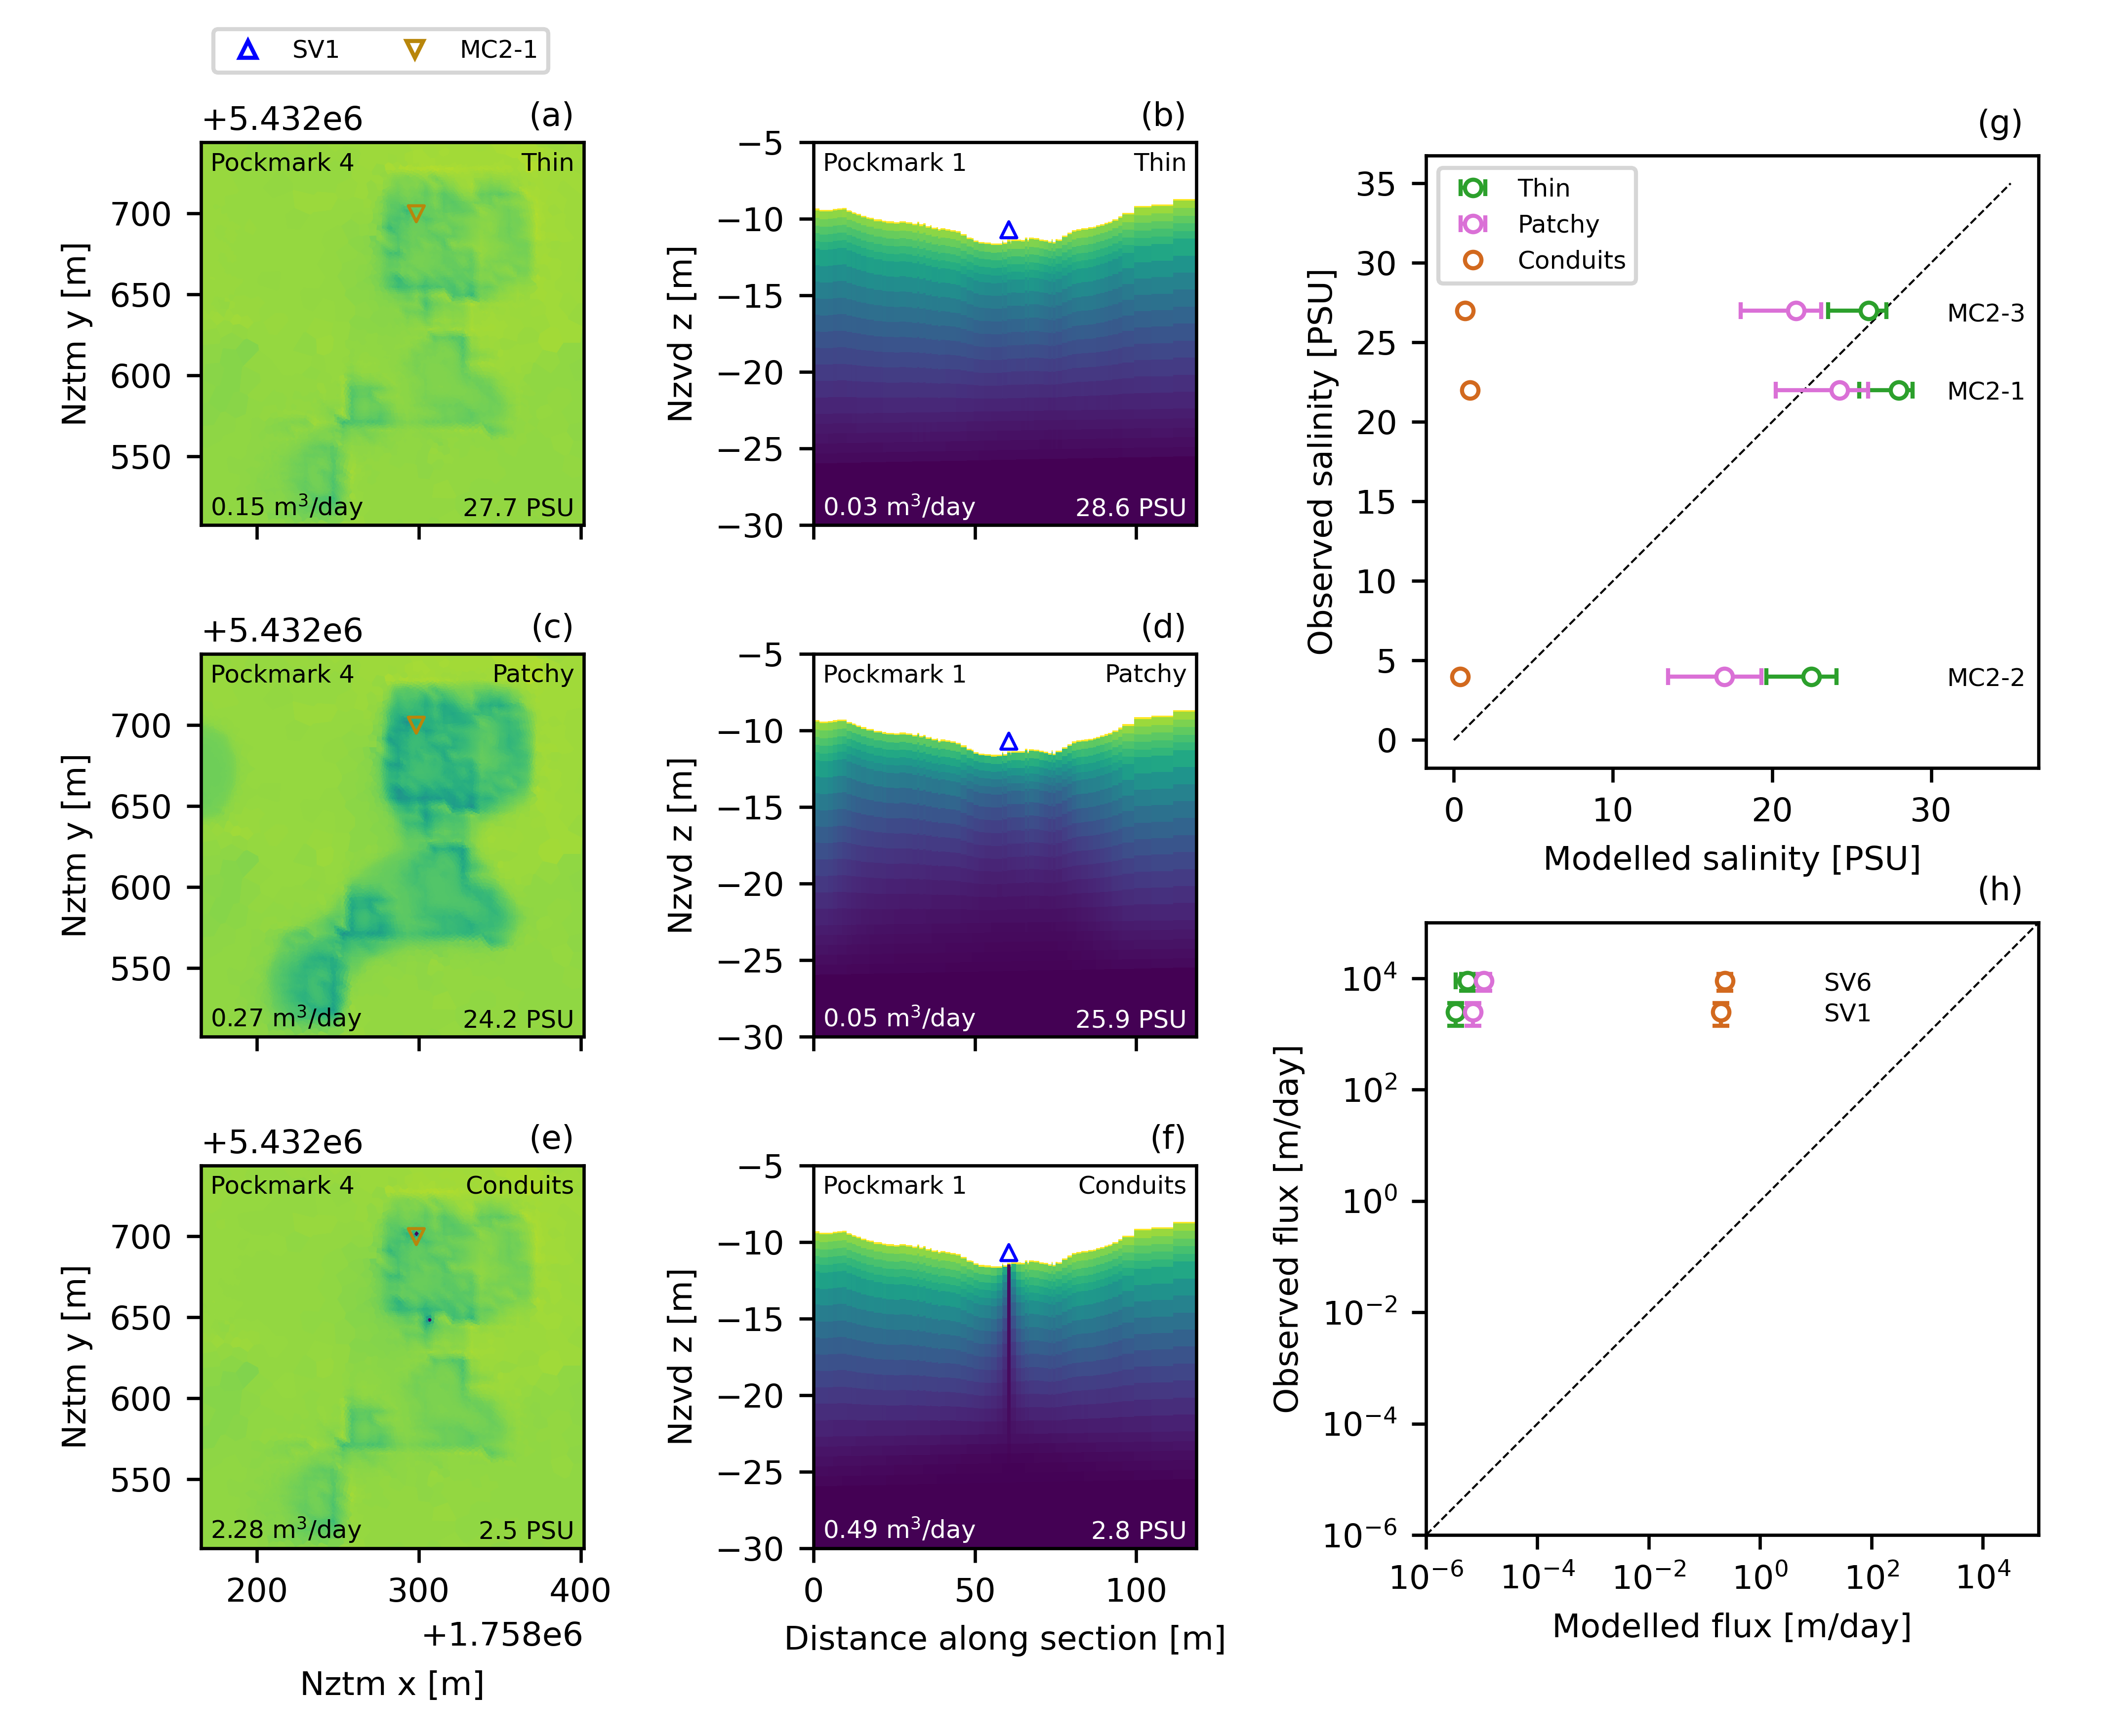
\includegraphics[width=1.25\textwidth]{alternate_hypotheses_pockmarks_and_model_vs_observed.png}}
\caption{The effects of different conceptual models of pockmark structure on groundwater salinity distributions, and comparison to observations. (a, c, e) Salinity in the top 0.5m of the Petone Marine Distal aquitard for Pockmark 4. (b, d, f) Sections showing salinity at Pockmark 1 (g) comparison between modeled and observed salinity in the top 0.5 m of the Petone Marine Distal aquitard for three locations. (h) comparison between modeled and observed flux at the two spring vents. For the Thin and Patchy Aquitard models, the error in the modeled value is taken as the range of salinities found within a ten-meter radius of the measurement.}
\label{fig:pockmark_comparison}
\end{figure}

The fit between modeled and observed salinities and fluxes varies across the three models (Figure \ref{fig:pockmark_comparison}g,h).
For the two salinity observations inside pockmarks, MC2-3 and MC2-1, where relatively saline water was observed,
the salinity in the uppermost cell of the Petone Marine Distal at the measurement point is close to the average salinity in the sediment core for the Thin and Patchy Aquitard models (Figure \ref{fig:pockmark_comparison}g).
The salinity at these points for the Aquitard Conduits model is much lower than the observed salinity.
This suggests that a high-conductivity pathway is not required to explain the salinity at these sampled points.
For the site outside of the pockmarks, MC2-2, where much lower salinity was observed,
the Thin Aquitard and Patchy Aquitard models do not give a good fit (Figure \ref{fig:pockmark_comparison}g).
The better match with the Aquitard Conduits model suggests that a more hydraulically conductive flow path may be present at this location.

The flux observed at SV1 and SV6 only comes closest to being reproduced by the Conduits model,
whereas the Thin Aquitard and Patchy Aquitard produce fluxes many orders of magnitude lower (Figure \ref{fig:pockmark_comparison}h).
This implies that conduits of some form could exist at these spring vents.

Fluxes and salinities at the observation points are expected to vary due to tidal forcing.
This may help to explain disparities between the observations and the model.
Model runs that included tidal forcing show that salinity at the observation points does not vary for the Thin Aquitard Model,
and varies slightly by around 0.01 PSU across the tidal cycle for the Aquitard Conduits Model (see Supporting Information Figures 4a and 5a).
This small variation would have little impact on the fit with the salinity observations (Figure 7g).
For the flux observation points, fluxes vary across the tidal cycle for both the Thin Aquitard and Aquitard Conduits Model (see Supporting Information Figures 4b and 5).
However, this tidal variation does not result in the orders-of-magnitude increase in flux that is required to match the model with the observations (Figure 7h).

Another process which was not included in the models was mechanical dispersion.
While dispersion is not expected to occur upgradient (downwards) from the seafloor boundary \cite{irvine_upstream_2021},
it could occur laterally from areas with greater downward dispersion around the measurement points.
Additional models were run to explore the potential effects of mechanical dispersion (see Supporting Information Figure 6).
Including mechanical dispersion increases the modelled salinity at the measurement points by up to around 5 PSU for the Thin Aquitard Model,
10 PSU for the Patchy Aquitard Model, and 6 PSU for the Aquitard Conduits Model.
For the Thin Aquitard Model and Patchy Aquitard model, this improves the fit with some of the observations and worsens the fit with others (Supporting Information Figure 6a,c).
For the Aquitard Conduits Model, this improves the fit for all observations (Supporting Information Figure 6f).
Including dispersion has no effect on the flux at the measurement points (Supporting Information Figure 6b,d,f).

The fit between each model and the observations is sensitive to the hydraulic properties assigned to the patches and conduits, which are themselves uncertain.
A modest increase in patch conductivity, or a lower conduit conductivity, would move the modelled salinities and fluxes toward or away from individual observations.
The comparisons presented here are therefore a first-order assessment of which conceptual model is most consistent with each observation,
rather than as a calibration of specific parameter values.

\subsection{Response of pockmarks to aquifer depletion and sea-level rise}

Prior to presenting the scenario results, we summarise how well the three models match the available observations.
We did not formally calibrate the models to the pockmark data, rather, the aquitard properties come from the calibrated regional model (Section 3.2).
We prescribed the patch and conduit properties rather than fitting them.
This is because there are only five point observations, three salinities and two fluxes and both the measurements and their locations carry substantial uncertainty (Section 3.6).
For this reason we determined that a formal calibration is not warranted.
Instead, we assess consistency qualitatively.
The Thin and Patchy Aquitard models reproduce the two saline core salinities inside the pockmarks (MC2-1 and MC2-3) within their observed range.
However, they underpredict (by orders of magnitude) the low salinity at MC2-2 and the spring-vent fluxes.
The Aquitard Conduits model reproduces the low salinity at MC2-2 and comes within an order of magnitude of the spring-vent fluxes.
By contrast, it overpredicts the freshening at MC2-1 and MC2-3.
As such, no single model matches all five observations.
This suggests the aquitard is heterogeneous across the study area.
Given this level of consistency, we use the models to explore how the pockmarks respond to aquifer depletion and sea-level rise.
To be clear, these scenarios are exploratory, not predictive.
The differences between the three models are expected to bound the range of plausible responses.

The response of groundwater flow and salinity distribution at pockmarks to sea-level rise and aquifer depletion depends on the geological model used to model the pockmark features. 
Flow under the pockmarks is reversed during the aquifer depletion scenario for all models (Figure \ref{fig:pockmarks-response}b,e,h).
However, the low hydraulic conductivity of the Petone Distal unit means that the salinity distribution beneath the pockmarks does not noticeably change during a one-year period of a reversed hydraulic gradient {for the Thin and Patchy Aquitard models (Figure \ref{fig:pockmarks-response}b and e).
For the Aquitard Conduits model, seawater intrusion does occur down into the aquifer through the conduits, causing salinization (Figure \ref{fig:pockmarks-response}h).
For all models, if mechanical dispersion was included, the amount of seawater intrusion would be expected to be greater \cite{werner_seawater_2013}.

\begin{figure}[h!]
\centering
\makebox[\textwidth][c]{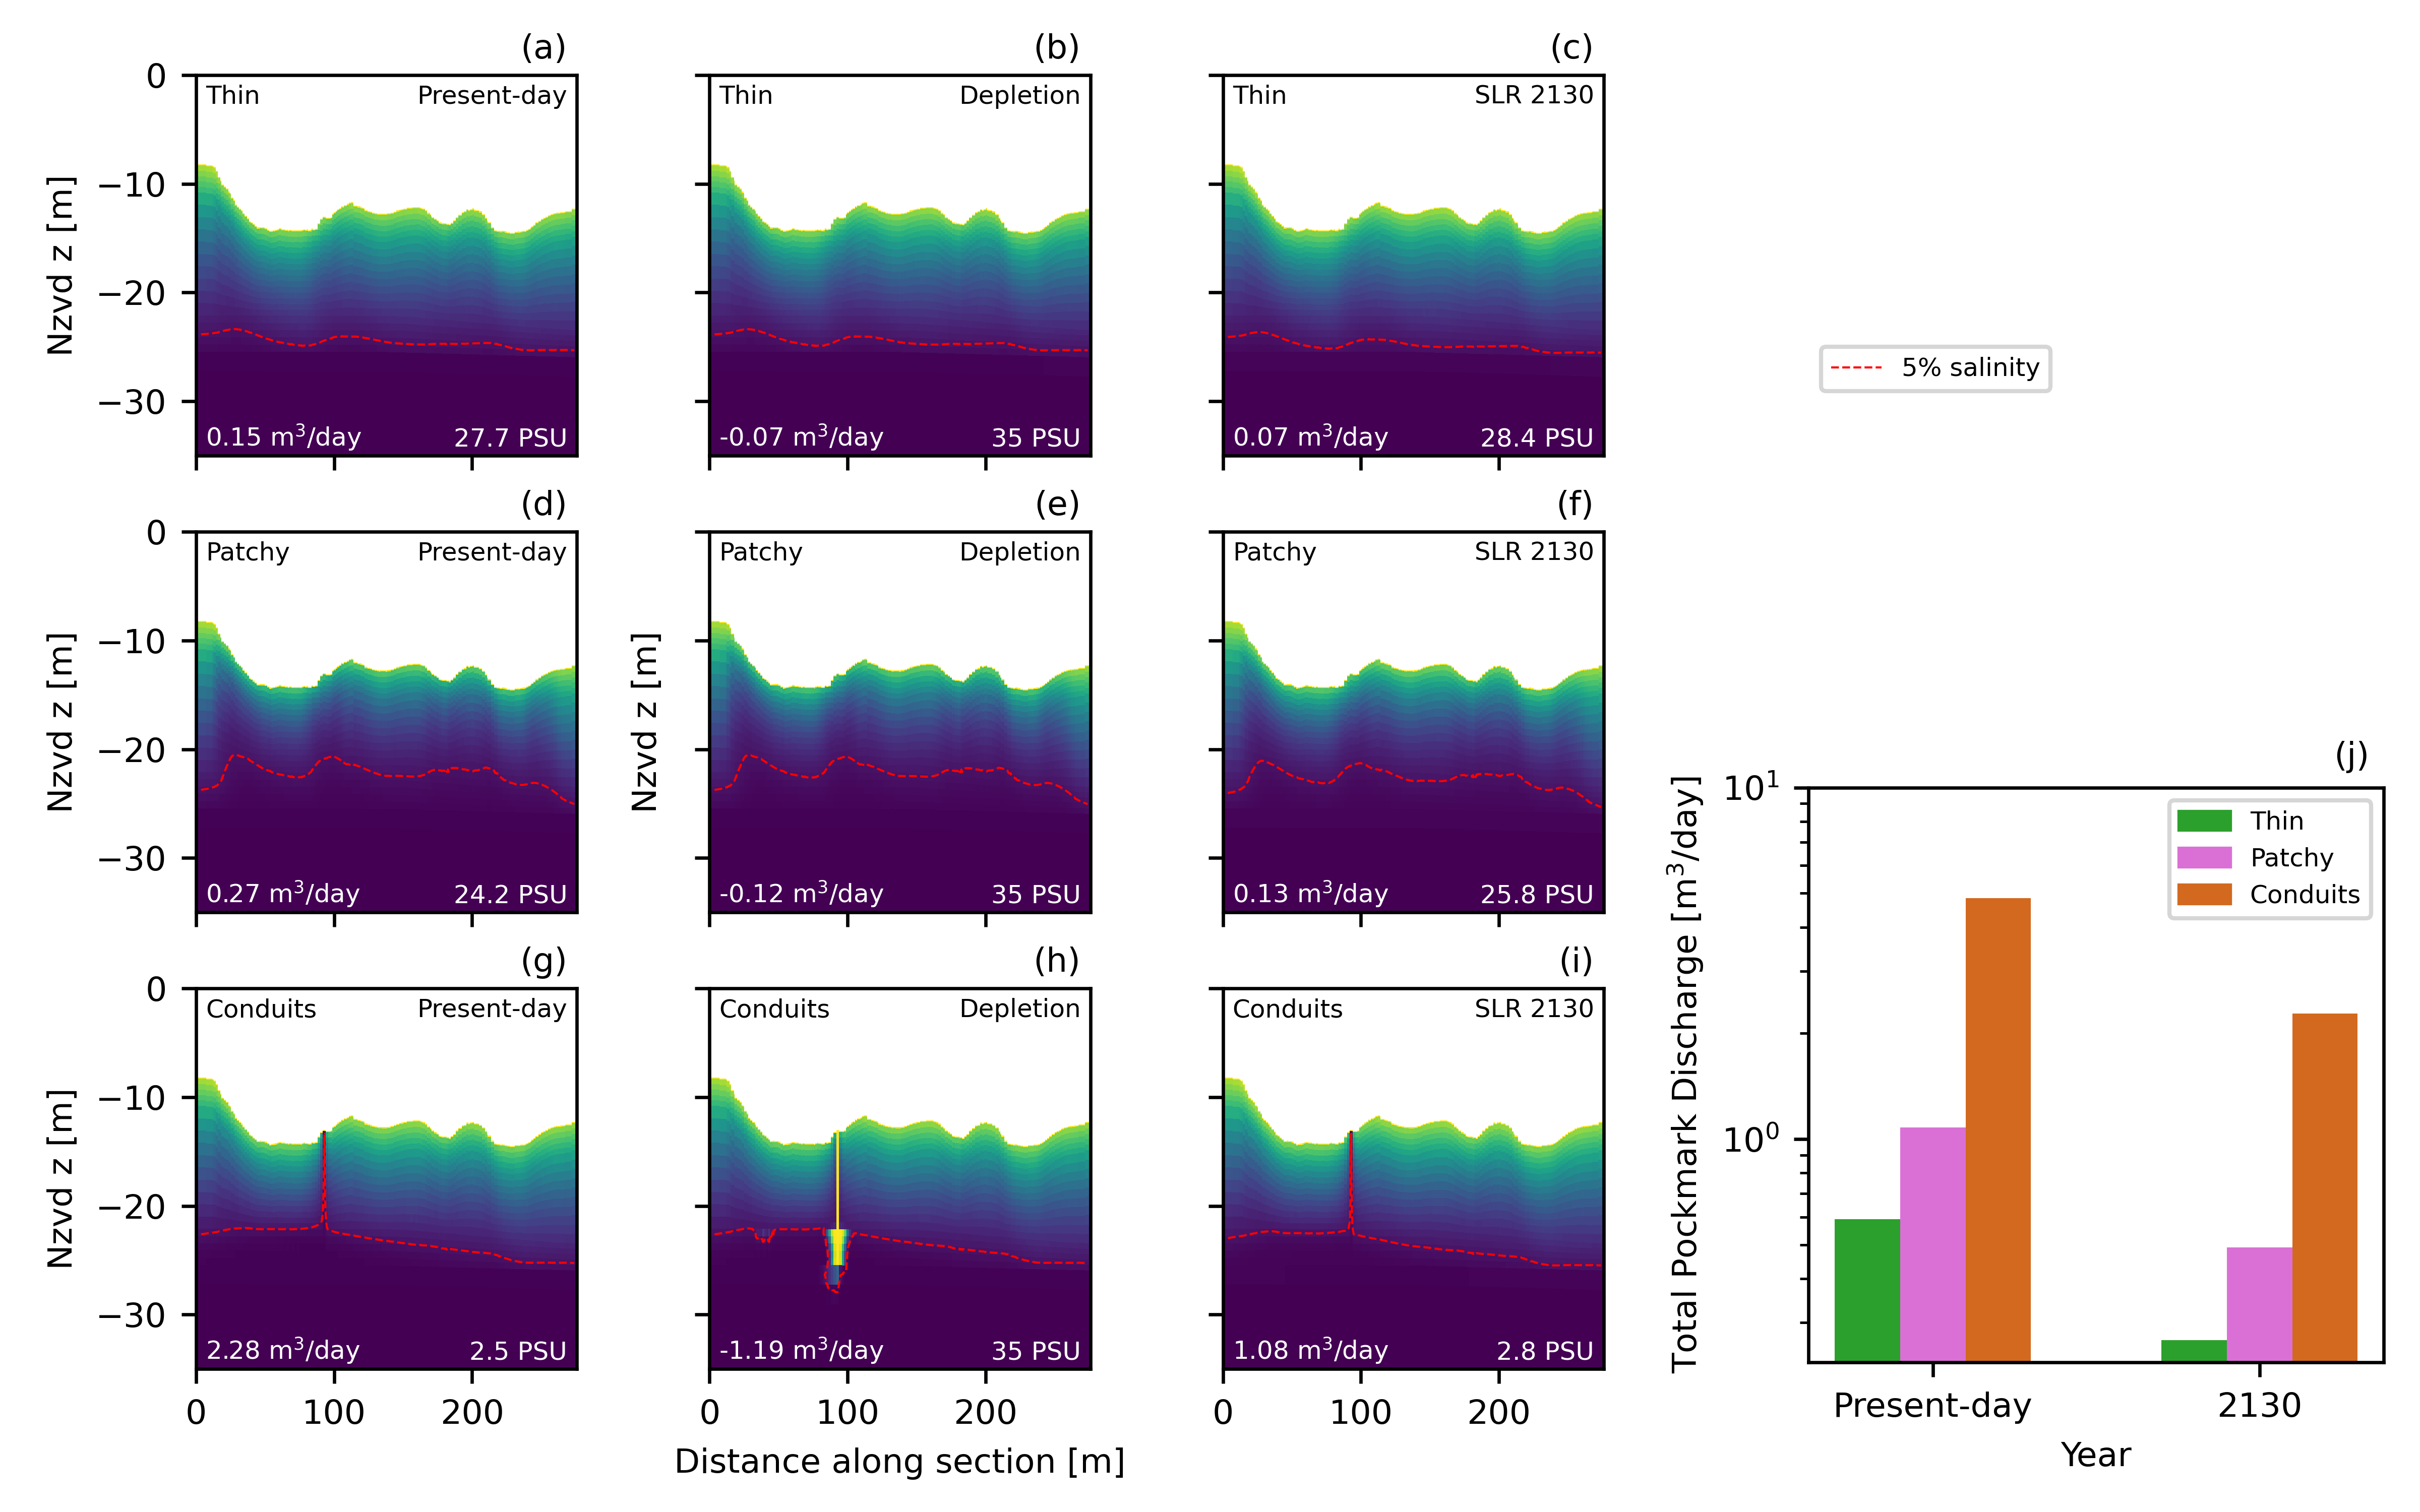
\includegraphics[width=1.3\textwidth]{alternative_hypotheses_changes.png}}
\caption{(a-i) Salinity distribution and discharge rates at Pockmark 3 for the Thin Aquitard Model, the Patchy Aquitard Model, and the Aquitard Conduits model for the present-data, aquifer depletion, and sea-level rise scenarios. (j) Total pockmark discharge for the present-day and sea-level rise (2130) scenarios.}
\label{fig:pockmarks-response}
\end{figure}

Under sea-level rise, the discharge at the pockmarks is reduced (e.g. Figure \ref{fig:pockmarks-response}c),
and the aquitards become more saline due to less advection opposing downward diffusion (Figure \ref{fig:pockmarks-response}c, f, i).
The absolute change in groundwater discharge at the pockmarks depends on the model (Figure \ref{fig:pockmarks-response}j).
However, the relative change in discharge is similar. For the Thin Aquitard model, pockmark discharge decreases by 54\% from 0.59 to 0.27 m$^3$/day.
For the Patchy Aquitard model, pockmark discharge also decreases by 54\% from 1.08 to 0.49 m$^3$/day.
For the Aquitard Conduits model, pockmark discharge decreases by 52\% from 4.8 to 2.3 m$^3$/day.
This corresponds closely to the decrease in hydraulic gradient between the onshore aquifer boundary ($h_{\mathrm{on}}$), and the seafloor ($h_{\mathrm{sea}}$),
which is around 50\% (Table \ref{tab:table_stages}).

\section{Discussion}

\subsection{Groundwater flow and transport at pockmarks}
The characteristics of groundwater discharge at pockmarks depend on their geometry and hydraulic properties.
We found that the greatest discharge occurs inside the edges of the pockmarks, as well as locations where the hydraulic conductivity of the aquitard is increased, such as at conduits.
The freshest discharge was found at the edges of pockmarks or, in the case of Pockmark 6, at the point where the aquitard was thinnest, as well as in the conduits.
This is consistent with findings from the modelling studies of \citeA{kaleris_modelling_2002} and \citeA{mulligan_role_2007}, who both observed greater flow at the edges of preferential flow features.
While both of these studies represented preferential flow features using increased hydraulic conductivity,
we observed this effect when pockmarks were represented using realistic bathymetry that reduced the thickness of an underlying aquitard with a homogeneous hydraulic conductivity (Figure \ref{fig_pockmarks_present_day}).
The observation of increased discharge at the edges of pockmarks may explain the formation of W-shaped pockmarks, such as those observed by \citeA{matciak_pockmarks_2024}.
It also relates to the observation of \citeA{harding_characteristics_2000} that spring vents were not only located in the centers of pockmarks.

We found that the modeled groundwater salinity within the pockmarks was lower than outside of them.
The magnitude of this difference depends on how much the pockmarks incise the aquitard, with fresher groundwater being found in deeper pockmarks.
When the hydraulic conductivity of the aquitard was increased below the pockmarks, this led to a further decrease in salinity.
Based on this, it is plausible that sampling the salinity of pockmarks could be used to identify the presence of offshore fresh groundwater \cite{hoffmann_fresh_2023, hoffmann_complex_2020}.
However, this is only likely to be effective where the offshore fresh groundwater is actively being discharged, and the advective flow rate is sufficient to prevent over-dominant diffusion \cite{micallef_offshore_2021}.
Our results suggest that samples taken in the deepest points of pockmarks, such as the base of Pockmark 6, or on the edges of the flatter bases of pockmarks,
may be more likely to encounter low salinities. Additionally, areas of pockmarks where the seafloor texture is softer may be indicative of groundwater discharge \cite{harding_characteristics_2000, hoffmann_fresh_2023}.

We did not observe convection cells such as those seen by \citeA{kaleris_modelling_2002} and \citeA{mulligan_role_2007} in some of their simulations.
This is possibly caused by either too low hydraulic conductivity, or too high vertical flux preventing the onset of free convection \cite{greskowiak_tideinduced_2014}.
Additionally, the complex bathymetry may also dissipate any convective effects \cite{simmons_variable-density_2001}.
Further work could compare a model where pockmarks are represented through bathymetry, such as presented here,
with a model where pockmarks are represented parametrically by increasing the hydraulic conductivity of cells where they are located \cite{kaleris_modelling_2002},
for the same site.
his would help determine whether model abstraction may cause the erroneous occurrence of free convective cells.

Comparing the results for three different pockmark geological models to the available discharge and salinity measurements, we are able to capture some of the observations.
Two of the salinity measurements of \citeA{hoffmann_fresh_2023} were consistent with the Thin Aquitard model results,
and this fit was improved slightly with the Patchy Aquitard model (Figure \ref{fig:pockmark_comparison}).
The Aquitard Conduits model best explains the very fresh observation at MC2-2, which was taken in the space between pockmarks,
where anomalous salinity and turbidity were detected in the water columns \cite{hoffmann_fresh_2023}.
However, if the aquitard hydraulic conductivity was increased by a larger factor of 100 in the Patchy Aquitard model $(K_v=1.8\times10^{-3} \mathrm{m/day})$,
then this could also explain the observed salinity at MC2-2  (Supporting Information Figure 7).
This indicates that this observation is not necessarily associated with a conduit or similar preferential flow path.

The high discharge fluxes observed at the spring vents by \citeA{harding_characteristics_2000}, and the narrow turbidity plumes observed by \citeA{hoffmann_fresh_2023} are most consistent with the Aquitards Conduit model.
None of the results of the three geological models were consistent with the flux measurements, and the total flux through all of the pockmarks was on the order of 1 m$^3$/day for the Aquifer Conduits model, which had the most discharge.
This is also significantly less than estimates of groundwater discharge at the pockmarks from regional modeling, 3000 m$^3$/day, across five areas with pockmarks in the harbour \cite{bennett_hutt_2024}.
However, this is water-balance output of a regional-scale model and carries substantial uncertainty, and it integrates over several pockmark areas rather than the single cluster modelled here.
Hence, it should be considered an order-of-magnitude reference rather than an exact target.
Increasing the vertical hydraulic conductivity of the conduits would increase these fluxes.
However, to match the magnitude of discharge, the vertical hydraulic conductivity of the conduits would likely need to be between 100 m/day and 1000 m/day.
This would be very high for the silt and sand Petone Marine hydrostatic units, which still appear to be present beneath the incised pockmarks (Figure \ref{fig:pockmarks_info_composite}b).
Additionally, given that the velocities measured at the spring vents are larger than the typical values reported in the literature, it is difficult to make any strong conclusions about the hydraulic conductivity of the preferential flow paths associated with the springs.
Further sampling at the spring sites, such as the combined use of seepage meters and Amphibian Electrical Resistivity Tomography (AERT), may provide more reliable measurements of discharge rates to validate this \cite{diego-feliu_combining_2025}.

The discharge across the seafloor (including the pockmarks) in the Thin Aquitard model is around 13.5 m$^3$/day (Figure \ref{fig_pockmarks_present_day}a),
whereas discharge through an individual conduit (as represented in the Aquitard Conduits model) is on the order of 1 m$^3$/day (Figure \ref{fig:pockmarks-response}g).
However, given that the exact properties of preferential flow paths in the study area are not constrained, this number is highly uncertain.
Furthermore, it is unknown how extensive preferential discharge is across the rest of the harbour.
Given the significant uncertainty in pockmark discharge, it is difficult to determine whether diffuse or focused submarine groundwater discharge is more significant in the model area.

One physical process that is omitted from the model is tidal forcing.
However, additional model runs including tidal forces show that tidal variation cannot explain the differences between the modelled salinities and fluxes with the observations of \citeA{hoffmann_fresh_2023} and \citeA{harding_characteristics_2000} (Supporting Information Figures 4 and 5).

Including mechanical dispersion in the model would slightly increase the modelled salinity at the measurement points (Supporting Information Figure 6).
The general differences between the fit of the three conceptual models with the salinity observations are similar to those when mechanical dispersion is not included.
If mechanical dispersion was responsible for high salinity at observations, and this was ignored during model calibration,
this could result in an underestimation of vertical hydraulic conductivity. Subsequently, model predictions could underestimate seawater intrusion.

\subsection{Implications for seawater intrusion and the vulnerability of offshore groundwater}

Focused discharge through the pockmarks is a small part of the offshore water budget.
The six modelled pockmarks discharge 0.59 m³/day in the Thin Aquitard model, around one percent of the discharge across the offshore model boundary.
For the Aquitard Conduits pockmark discharge is around 4 m³/day.
This is still well below the regional estimate for all pockmark areas.
This is because diffuse discharge across the broader seafloor likely dominates the freshwater flux, rather than the pockmarks themselves.
For this reason, the significance of the pockmarks lies less in discharge volume, and more in the pathways they may provide for seawater intrusion, and their local influence on seafloor salinity and the ecosystems it supports.

In the Wellington Harbour, the largest concern around pockmarks is the potential for seawater intrusion into the aquifer due to reversed spring flow.
After one year of an extreme aquifer depletion scenario, our results show saline groundwater reaching the Upper Waiwhetū aquifer only in the Aquitard Conduits model (Figure \ref{fig:pockmarks-response}).
No intrusion occurred in the Thin and Patchy Aquitard models.
This is because, in both of these models, the aquitard vertical hydraulic conductivity within the pockmarks is low,
resulting in a slow advection of saline groundwater down into the aquifer.
However, if the vertical hydraulic conductivity of the aquitard patches was greater, and aquifer depletion was sustained for a longer time, saline groundwater could enter the Upper Waiwhetū aquifer (Supporting Information Figure 8).

Seawater intrusion through pockmarks is not only a problem for the salinization of onshore groundwater resources.
With the recent focus on offshore fresh groundwater as a water resource \cite{bakken_submarine_2012, zamrsky_offshore_2022},
salinization of offshore groundwater through pockmarks may be a limiting factor for its exploitation \cite{gyopari_wellington_2018}.
Given the occurrence of pockmarks in a number of offshore freshened groundwater hotspots (Figure \ref{fig:pockmarks_global_map}),
understanding the potential for seawater intrusion through pockmarks is crucial.
Therefore, it is essential to characterize the heterogeneity of the aquitard and its influence on submarine groundwater discharge at pockmarks to assess the vulnerability of offshore fresh groundwater through them.

The identification of pockmarks and conduits to flow associated with them may prove a challenge to quantifying the risk they pose to a coastal aquifer system.
The findings of \citeA{hoffmann_fresh_2023} show that high hydraulic conductivity flow paths exist in the area of the Hutt River pockmarks that are not necessarily located inside of the pockmarks.
These flow paths pose less of a seawater intrusion threat than high hydraulic conductivity flow paths within pockmarks. This is because the
equivalent freshwater head in the saline aquitard is greater at the deeper points of the seafloor due to the density of the water column.
Consequently, the head in the fresh aquifer requires less of a reduction to reverse the equivalent freshwater head gradient and resulting flow \cite{post_variable_2022}.
However, the fact that such flow paths do not have an obvious surface expression may make their identification difficult, compared to flow paths within pockmarks. As a result,
they may go unnoticed and lead to unexpected salinization.

In the Wellington Harbour, the relatively small area over which the aquifer system extends offshore has facilitated the collection of high-resolution bathymetry data,
meaning all pockmarks in the area have been identified \cite{hoffmann_fresh_2023}. In larger offshore environments such as continental shelves,
some of which hold large reserves of offshore fresh groundwater \cite{zamrsky_offshore_2022}, the identification of pockmarks and the risk of salinization through them will be more difficult \cite{goff_modern_2019, gustafson_aquifer_2019}.
This is because seismic surveys taken as transects of the system are only likely to encounter a small number of the existing pockmarks \cite{bertoni_seismic_2020}.
Furthermore, buried pockmarks that have been infilled with coarser sediment may be difficult to identify  \cite{goff_modern_2019}.
Buried pockmarks may form connections between aquifers. This connection may result in the salinization of deeper fresh aquifers from saline groundwater in shallower aquifers.

Two aspects of the depletion response are not resolved by the single scenario presented here.
The first is reversibility.
Whether saline groundwater that entered the aquifer through a conduit would be flushed out once a seaward gradient was restored, and how this depends on the duration of the reversal.
The second is the dependence on the depth and duration of depletion.
The Aquifer Depletion Scenario shows that intrusion through pockmarks is possible in principle where conduits are present, but the head reduction and its persistence required to salinise the aquifer at a given site remain to be quantified.
These are general questions for coastal systems that contain pockmarks, and are not specific to the Wellington Harbour.
Seawater intrusion and subsequent recovery through preferential flow features in sub-seafloor aquitards is an important topic for future research.
A generalized study which explores the effect of preferential flow feature properties, and the magnitude and duration of aquifer depletion on seawater intrusion and recovery would be useful for understanding the vulnerability of coastal aquifers to salinization.

\subsection{Effects of sea-level rise on pockmark discharge}
The reduction in submarine groundwater discharge at pockmarks depends on the hydraulic properties of the aquitard within the pockmarks.
For all three geological models, we found the projected sea-level rise will decrease the pockmark discharge by over 50\% by 2130 (Figure \ref{fig:pockmarks-response}j).
This is a result of surface drainage in the Hutt Valley, which causes the system to be partially topographically-limited \cite{bennett_hutt_2024, michael_global_2013}.
Submarine groundwater discharge driven by seaward hydraulic gradient may cease following a smaller magnitude of sea-level rise at pockmarks than the seafloor around them.
This is because of the increased equivalent freshwater head in the seafloor beneath the pockmarks \cite{post_variable_2022}.
This means the impact of sea-level rise on coastal groundwater discharge may be greater in systems that feature pockmarks.
The absolute reduction in discharge depends on the geological structure of the pockmarks and is greatest when conduits exist within them (Figure \ref{fig:pockmarks-response}j).

This further emphasizes the importance of identifying preferential flow paths through seafloor aquitards. If the coastal groundwater level is not able to rise with the sea level,
pockmark discharge will decrease.
While previous studies have not reported the occurrence of submarine groundwater discharge-dependent ecosystems at pockmarks in the Wellington Harbour,
pockmarks and submarine springs are hotspots for such ecosystems in other locations \cite{purkamo_impact_2022, idczak_geophysical_2020, taniguchi_submarine_2019}.
If sea-level rise caused a decrease in discharge in these locations, their ecosystems may be negatively impacted.
The presence of drains in coastal aquifer systems increases the impact of sea-level rise on submarine groundwater discharge and seawater intrusion vulnerability \cite{michael_global_2013, morgan_sea-level_2024, seibert_understanding_2024}.
The presence of pockmarks will exacerbate these impacts.

\subsection{Persistent geological uncertainty}

A central limitation of this study is that the available observations cannot uniquely constrain the property that matters most for both discharge and intrusion,
the vertical hydraulic conductivity, spatial extent, and number of preferential flow paths through the aquitard.
The low salinity at MC2-2, for example, can be reproduced either by a discrete conduit or by increasing the patch conductivity by a factor of one hundred (Supporting Information Figure 7).
Equally, an apparently saline core does not exclude a nearby conduit,
because a small number of cores may not intersect localized high-conductivity paths whose extent is on the order of metres \cite{hoffmann_fresh_2023}.
The inference that no conduit is present at MC2-1 and MC2-3 should therefore be read as a statement about the sampled locations rather than the pockmarks as a whole.
This non-uniqueness is the main barrier to quantifying seawater intrusion risk at the pockmarks, which could be reduced by additional data collection and analysis.

The presence of submarine springs poses a challenge to understanding groundwater discharge at seafloor pockmarks,
as they represent high-permeability flow paths that are difficult to characterize and represent in a model.
Collecting conductivity profiles using geophysical methods such as controlled-source electromagnetic \cite{gustafson_aquifer_2019, micallef_3d_2020},
or continuous resistivity profile methods \cite{becker_locating_2023}, would help improve understanding of the distribution of fresh submarine groundwater discharge.
Such profiles should be recorded along different pockmark transects,
where submarine groundwater discharge had already been identified through anomalies in water-column measurements such as salinity and turbidity \cite{hoffmann_fresh_2023}.
These profiles could be supplemented by cone penetration testing (CPT) within and around the pockmarks to characterize the sediment properties,
and any associated heterogeneity}\cite{reusch_giant_2015}.
To further understand the effect of tidal dynamics on discharge, continuous salinity and acoustic doppler current profiler (ADCP) measurements could be taken} \cite{poulsen_detecting_2015}.
The collection of such data may allow for the development of a stochastic representation of aquitard heterogeneity \cite{van_leer_investigating_2025}.
This would facilitate more robust analysis of seawater intrusion vulnerability.

Another significant source of uncertainty in our methodology is associated with the extent and contact surfaces of the hydrostratigraphic units.
The numerical model used is based on a hydrostratigraphic model that uses deterministic interpolation of discrete measurements \cite{begg_revised_2023}.
A different interpolation of these measurements could change how much the thickness of the Petone Marine Distal aquitard was reduced at the pockmarks, influencing the groundwater flow and transport conditions.
Using a stochastic representation of hydrostratigraphic units would help to quantify this uncertainty \cite{de_la_varga_gempy_2019, haehnel_development_2024, bardot_seamless_2025}.

If these geological uncertainties could be accounted for and a model of aquitard heterogeneity were developed that reproduced both flux and salinity measurements in the study area,
a logical next step would be to incorporate this information into the regional model.
This could either be through local grid refinement \cite{hughes_flopy_2024}, model splitting/nested models,
or through upscaling the results, potentially by finding the average flux across the area of regional model cells and calculating an effective vertical hydraulic conductivity \cite{van_leer_estimating_2023}.
One limitation of using an upscaled model is that the initial onset of seawater intrusion through the pockmarks would not be captured,
as the lowest points of the bathymetry where the hydraulic gradient is most easily reversed would be smoothed out in the averaging process.

\section{Conclusions}
We have modeled groundwater discharge at pockmarks with greater spatial resolution than previous studies.
This has enabled an in-depth comparison with observations of submarine groundwater discharge in the Wellington Harbour, New Zealand.
Our modeling supports the current conceptualization that preferential flow is an important aspect of the offshore groundwater system and provides insights into the nuances surrounding submarine groundwater discharge within pockmarks.
We found that if the hydraulic conductivity of the aquitard in which pockmarks are incised is homogeneous, submarine groundwater discharge fluxes may be up to 2.5 times greater,
with salinities reduced by up to 25 \% in the pockmarks,
compared to the seafloor around them.
Within the pockmarks, the greatest discharge and lowest salinities are found at the center of narrow pockmarks or on the edges of pockmarks with flatter bases.
These may be good locations to sample or detect the presence of submarine groundwater discharge and offshore fresh groundwater.
Consistent with the observations, conduits or spring vents at the pockmarks, with sufficiently high hydraulic conductivity, could correspond to the highest submarine groundwater discharge rates, and potentially lead to the most consequential seawater intrusion if flow was reversed.
Identifying these flow paths is critical for quantifying the risk of salinization through pockmarks, which have implications for the use of offshore fresh groundwater as a resource.
Further understanding of groundwater flow at pockmarks could be gained by applying this methodology to other sites, and combining such modeling with additional observations, such as geophysical profiles, would greatly reduce the uncertainty surrounding them.

\section*{Open Research Section}
The Python scripts used to build, run, and postprocess the groundwater models in this manuscript are available in the GitHub repository at \url{https://github.com/connorcleary/pockmark_modelling} \cite{cleary_python_2025}. The required grid files to build these groundwater models, and example MODFLOW6 input and output files for the Present-day scenarios presented in this manuscript are available at \url{https://doi.org/10.5281/zenodo.17300482} \cite{cleary_grid_2025}.


\section*{Conflict of Interest declaration}
The authors declare there are no conflicts of interest for this manuscript.

\acknowledgments
The authors would like to acknowledge Wellington Water Ltd. and the Greater Wellington Regional Council for granting the use of the RLHGM and the outputs of HAM5, Sam Davidson from NIWA for providing the multibeam bathymetric data, Joshu Mountjoy for his feedback and suggestions on the study, and Jaspar Hoffman for providing the sediment core data. Thank you to Janek Greskowiak and Catherine Moore for reviewing an early version of the manuscript. Connor Cleary would like to acknowledge the support of the University of Canterbury Doctoral Scholarship, under which this research was conducted. Leanne Morgan is supported by Canterbury Regional Council, New Zealand, and the New Zealand Ministry of Business, Innovation and Employment Future Coasts Funding Contract C01X2107. % todo thank named reviewer

\bibliography{references}

\end{document}
